%! Unused graphs



%!fORMAT IMAGE FULL PAGE

%!% CICA tables and function
    %Table PI table, Function1, CICA evaluation process on architectural facades. Table 1x3
    \begin{table*}[!htb]
    \centering
    \small
    \begin{tabular}{c}
        %Top cell with one figure
        %Table: Performance Indicators
        \begin{minipage}{\textwidth}
            \centering
            \captionof{table}{Table of Metrics and Weights for Complexity Scoring: Outlines the key criteria and corresponding weights utilized in the Computational Image Complexity Analysis (CICA) to determine the `Complexity Score' of architectural facades, detailing the systematic approach to quantifying facade intricacy through edge density and contour count metrics.}
            \label{tab:MetricsandWeights}
            \begin{tabularx}{\textwidth}{p{2.5cm} p{1cm} X X p{1cm}}
                \toprule
                \multicolumn{5}{c}{\textbf{Table of Metrics and Weights for CICA Complexity Scoring on Architectural Facades}} \\
                \toprule
                \textit{Complexity metric} &
                  \textit{N} &
                  \textit{Metric name/description} &
                  \textit{Quantitative   method} &
                  \textit{Weights} \\ \midrule
                \textbf{Edge Density} &
                  1 &
                  Edge detection using Canny Edge Detection algorithm for highlighting the most relevant features of a building.
                    &
                  Measured by dividing the number of non-zero (edge) pixels in the edges image by the total number of pixels in the image.
                    &
                  8\\
                \\
                \textbf{Contour count} &
                  2 &
                  Employs contour approximation algorithm for shape analysis to determine intricacy of edges.
                    &
                  Measure by counting the number of segments in an edge.
                    &
                  2\\ \bottomrule
                   &
                   &
                  \textbf{TOTAL} &
                  &
                  \textbf{10}\\ \bottomrule
            \end{tabularx}
        \end{minipage}
        \\
        \\
        \\
        %Middle cell with two nested figures side by side
        %Table function 1 complexity score
        \begin{minipage}{\textwidth}
            \centering
            \captionof{table}{Function 1: Complexity scoring function that integrates various criteria to assess the intricacy of a building facade.}
            \label{tab:ComplexityScoreFunction}
            \begin{tabularx}{\linewidth}{|X|}
                \hline
                \small
                \vspace{0.1cm}
                \multicolumn{1}{c}{\textbf{\(f_1\): Unified Complexity Scoring Function}}\\
                \textit{Calculate the complexity score for all images in the data pool.}
                \\ \\
                \begin{equation}
                    f_1(x) = \mathrm{round}\left(\sum_{i=1}^{n} w_i \cdot a_i, 2\right) = \text{complexity\_score}
                    \label{eq:F1_ComplexityScoreFunction}
                \end{equation}
                \\
                \textit{for the buildings included in the database.}
                \vspace{0.5em}

                \textit{where:}\\
                \(n\): number of performance indicators\\
                \(w_i\): weight of the \(i\)-th element\\
                \(a_i\): normalized score for the \(i\)-th metric (e.g., `Edge Density' and `Contour Count')\\
                \vspace{0.05em}
                \textit{Finally, the "Complexity Score" is assigned to each building for data visualization.}
                \vspace{0.5em}\\
                \hline
            \end{tabularx}
        \end{minipage}
        \\
        \\
        \\
        %Bottom cell
        %Table: CICA Image evaluation process for historical and 3d facades
        \begin{minipage}{\textwidth}
            \centering
            \captionof{table}{CICA Evaluation on Architectural Facades: The table presents a comparative analysis of CICA evaluation applied to 3D-modeled facades (a) and historical buildings (b). The process includes steps from original imagery to image processing (noise reduction, grayscale), edge detection, and contour count analysis, as shown on the flowchart in Figure\ref{fig:CICAImageEvaluationFlowchart}. It highlights  the adaptability of CICA to assess complexity in both historical and contemporary architectural designs.}
            \label{tab:CICAImageEvalProcessOnArchitecturalFacades}
            \begin{tabularx}
            {\textwidth}{X X X X }
                \toprule
                \multicolumn{4}{c}{\textbf{CICA Image Evaluation process on Architectural Facades}} \\
                \toprule
                \multicolumn{1}{c}{\textit{Original Image}} &
                 \multicolumn{1}{c}{\textit{Grayscale, noise reduction}} &
                \multicolumn{1}{c}{\textit{Edge detection Image}} &
                \multicolumn{1}{c}{\textit{Contour count Image}}\\
                \midrule
                \text{(a) 3D-modeled facades} &  &  &
                \\
                {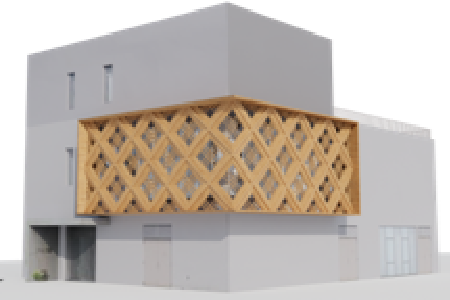
\includegraphics[width=1\linewidth]{Images/CICA3DRender1}} &
                    {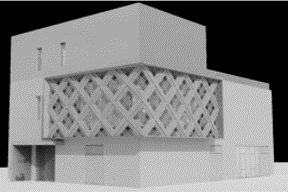
\includegraphics[width=1\linewidth]{Images/CICA3DRender2}} &
                  {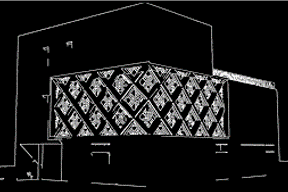
\includegraphics[width=1\linewidth]{Images/CICA3DRender3}} &
                  {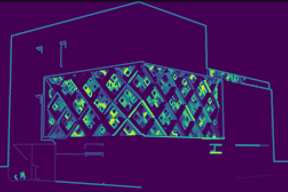
\includegraphics[width=1\linewidth]{Images/CICA3DRender4}} \\
                \midrule
                \text{(b) Historical Analysis} &  &  &
                \\
                {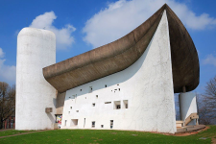
\includegraphics[width=1\linewidth]{Images/CICAHistory1}} &
                    {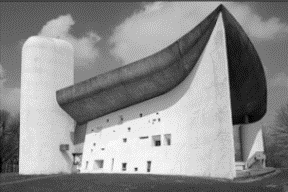
\includegraphics[width=1\linewidth]{Images/CICAHistory2}} &
                  {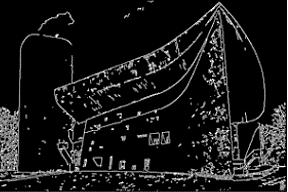
\includegraphics[width=1\linewidth]{Images/CICAHistory3}} &
                  {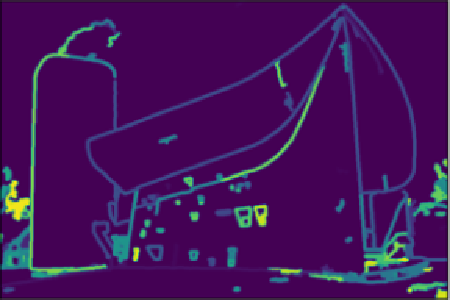
\includegraphics[width=1\linewidth]{Images/CICAHistory4}}\\
                \bottomrule
            \end{tabularx}
        \end{minipage}
    \end{tabular}
    \end{table*}


%!Survey tables
%% Participant background section table from survey
\begin{table}[htb]
    \centering
    \footnotesize
    \caption{Multiple choice survey for professional background}
    \label{tab:BackgroundSurvey}
    \begin{tabularx}{\linewidth}{p{0.125cm}X}
        \toprule
        & \textit{Participant background section. Multiple choice questions} \\
        \midrule
        1 & What is your current occupation? \\
        & a) Architect \\
        & b) Civil engineer \\
        & c) Construction manager \\
        & d) Urban planner \\
        & e) Other (please specify) \\
        \addlinespace
        2 & How many years of professional experience do you have in facade design? \\
        & a) None \\
        & b) Less than 1 year \\
        & c) 1--5 years \\
        & d) 6--10 years \\
        & e) More than 10 years \\
        \addlinespace
        3 & What is the highest level of education you have completed? \\
        & a) High school diploma \\
        & b) Associate degree \\
        & c) Bachelor's degree \\
        & d) Master's degree \\
        & e) Doctoral degree \\
        \addlinespace
        4 & Which software tools have you used for facade design? (Select all that apply) \\
        & a) AutoCAD \\
        & b) SketchUp \\
        & c) Revit \\
        & d) Rhino \\
        & e) ArcGIS \\
        & f) Other (please specify) \\
        \addlinespace
        5 & What challenges have you encountered when designing facades? (Select all that apply) \\
        & a) Limited space \\
        & b) Limited budget \\
        & c) Building program constraints \\
        & d) Client preferences \\
        & e) Environmental factors \\
        & f) Other (please specify) \\

        \bottomrule

    \end{tabularx}
\end{table}

%% Complexity perception section table from survey
\begin{table}[htb]
    \centering
    \footnotesize
    \caption{Complexity perception section  from survey for complexity analysis for facade design design}
    \label{tab:ComplexitySurvey}
    \begin{tabularx}{\linewidth}{p{0.125cm}X}
        \toprule
        & \textit{Complexity perception section. 7 - Likert scale} \\
        \midrule
        6 & To what extent do you find the overall complexity of this facade design appealing?\\
        & Strongly Disagree (1) —————— Strongly Agree (7) \\
        \addlinespace
        7 & How do you rate the intricacy of the patterns and textures used in this facade design? \\
        & Not Intricate at All (1) —————— Extremely Intricate (7)\\
        \addlinespace
        8 & To what extent do you think the arrangement of architectural elements on this facade adds to its visual interest? \\
        & Not at All (1) —————— Adds Significantly (7) \\
        \addlinespace
        9 & How complex do you perceive the facade's use of patterns and textures? \\
        & Not Complex at All (1) —————— Very Complex (7) \\
        \addlinespace
        10 & How detailed do you find the ornamentation on this facade design? \\
        & Not Detailed at All (1) —————— Extremely Detailed (7) \\
        \addlinespace
        11 & How much do the combination of materials contribute to the overall complexity of the facade? \\
        & Minimally (1) —————— Significantly (7) \\
        \addlinespace
        12 & To what degree does the composition of the facade strike you as aesthetically intricate? \\
        & Not Intricate at All (1) —————— Extremely Intricate (7) \\
        \addlinespace
        13 & How much do you believe that the arrangement of shapes and forms on the facade contributes to its complexity? \\
        & Not at All (1) —————— A Great Deal (7) \\
        \addlinespace
        14 & How significantly does the use of color enhance the facade's visual complexity? \\
        & Not Significantly (1) —————— Very Significantly (7) \\
        \addlinespace
        15 & How much depth and layering do you observe in the design of this facade? \\
        & None (1) —————— A Great Deal (7) \\
        \bottomrule
    \end{tabularx}
\end{table}

%! Function for complexity score
%%Table function 1 complexity score
\begin{table*}[htb]
    \centering
    \caption{Function 1: Complexity scoring function that integrates various criteria to assess intricacy of a building facade.}
    \label{tab:ComplexityScoreFunction_table}
        \begin{tabular}{|c c|}%{|c|c|}
        \hline
        % First Cell (Top-Left)
        % f1: Valid Position finder function
        \begin{minipage}{.49\linewidth}
            \centering
            \small
            \begin{tabular}{p{8cm}}
                \\
                \textbf{\(f_1\), Unified `Complexity Scoring' function 1}\\
                    \textit{Calculate the complexity score for all the images on the data pool}
                    \\
                    \begin{equation}
                        f_1(x) = \left[ \mathrm{round}\left(\sum_{i=1}^{n} w_i \cdot a_i, 2\right) \right] = complexity\_score
                    \label{eq:F1_ComplexityScoreFunction}
                    \end{equation}
                    \\
                    \textit{ for the Buildings included in the database.}\\
                \\
            \end{tabular}
        \end{minipage}
        &
        % Second Cell (Top-Right)
        % continuation f1
        \begin{minipage}{.49\linewidth}
            \centering
            \small
            \begin{tabular}{p{8cm}}
                \\\\
                \textit{where;} \\
                \(n \); is the number of performance indicators \\
                \(w_i \); represents the i-th elements weight input and \\
                \(a_i \); represents the i-th normalized score for the respective metric(`Edge Density' and `Contour Count').\\
                \\
                \textit{Finally, the `Complexity score' is assigned to each building for data visualization.}\\

            \end{tabular}
        \end{minipage}\\
        \hline
        \end{tabular}
\end{table*}


%!%Figures and table CICA
%Flowchart CICA, Figure of Cica on historical buildings and renders, PI table. Table 1x3
\begin{table*}[!htb]
    \centering
    \small
    \begin{tabular}{c}
        %Top cell with one figure
        %Figure Computational Image Compexity Analysis (CICA) System flowchart
        \begin{minipage}{\textwidth}
            \centering
            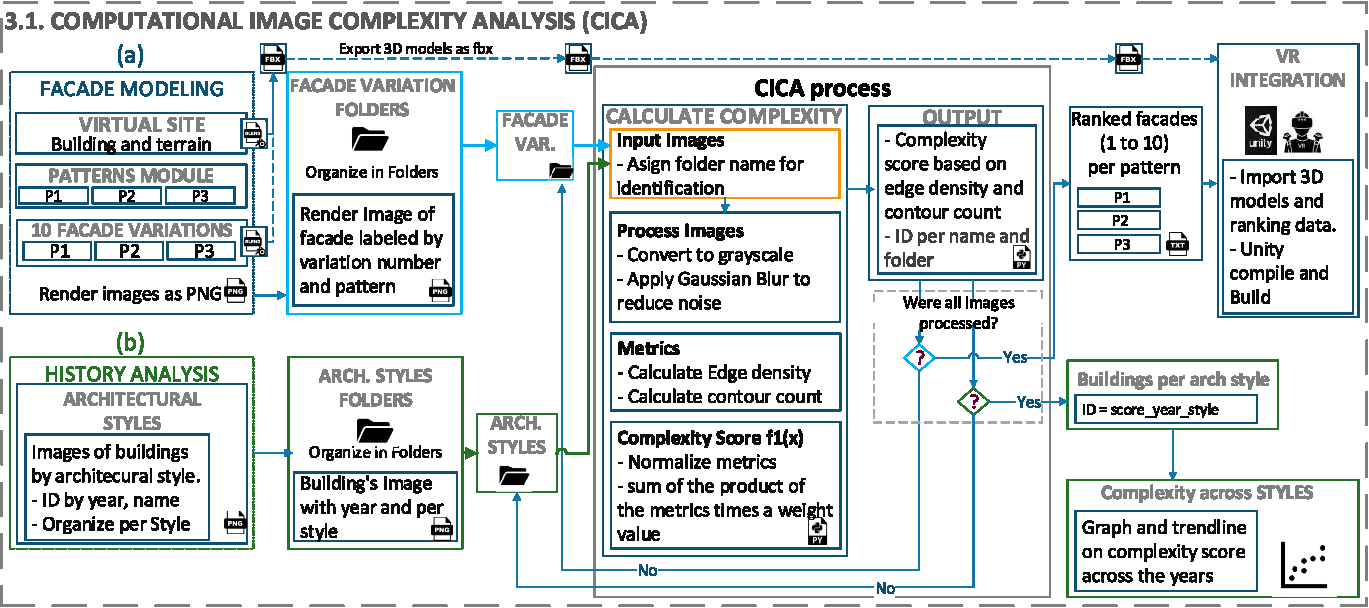
\includegraphics[width= \linewidth]{Images/CICAFlowchart}
            \captionof{figure}{Flowchart illustrating the applications of Computational Image Complexity Analysis system (CICA)(detailed in Section\ref{subsec:Computational Image Complexity analysis}), including its role in analyzing complexity scores for historical architectural styles and ranking of 3D modeled facades design with various degrees of complexity(presented in Section\ref{subsubsec:CICAforFacades}).}
            \label{fig:ImageComplexityAnalysisFlowchart}
        \end{minipage}
        \\
        \\
        %Middle cell with two nested figures side by side
        %%%Figure CICA on historic buildings and renders. Table 1x2
        \begin{minipage}{\textwidth}
            \centering
            % Left figure
            \begin{minipage}{0.49\textwidth}
                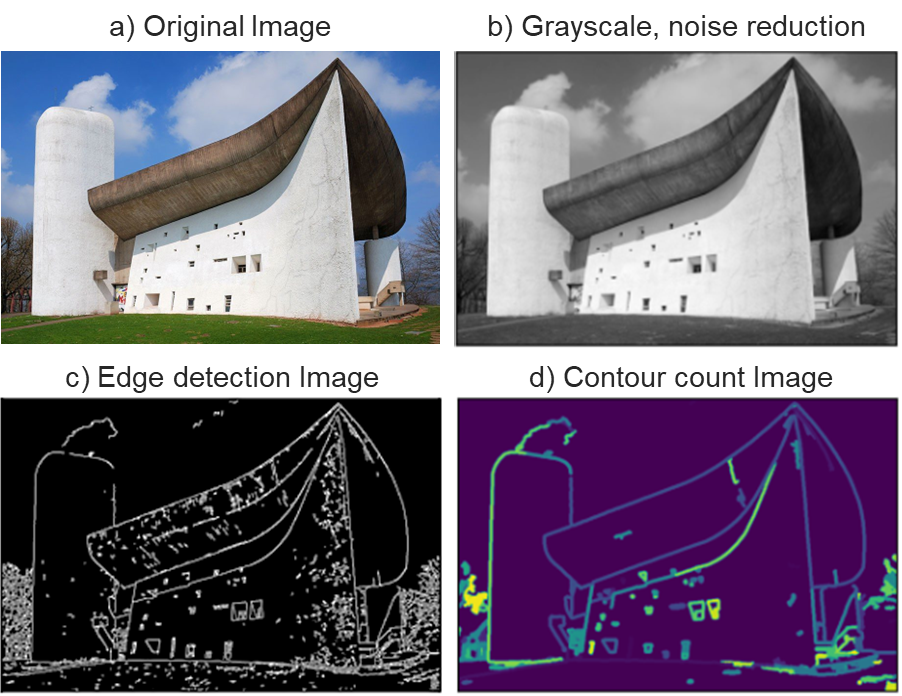
\includegraphics[width= \linewidth]{Images/CICAHistoryPlot}
                \captionof{figure}{CICA evaluation on historical Buildings: Illustration showcasing steps from original imagery to Image process, Edge Detection and Contour Count analysis. This process underpins the complexity assessment of facades, highlighting the analytical depth of CICA in quantifying architectural intricacies.}
                \label{fig:CICAHistoryPlot}
            \end{minipage}
            \hfill % Spacing between the figures
            % Right figure
            \begin{minipage}{0.49\textwidth}
                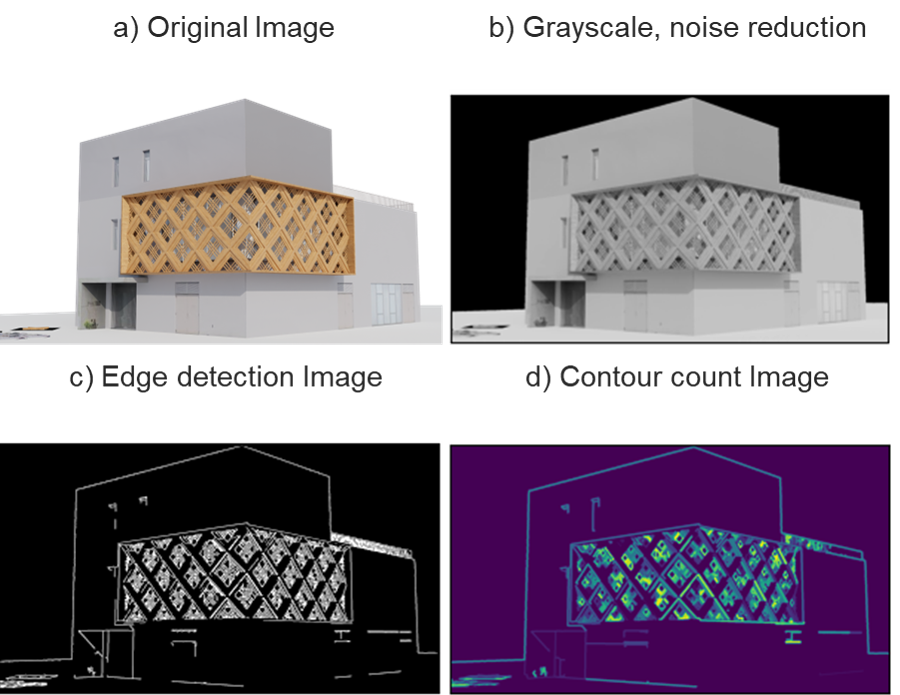
\includegraphics[width= \linewidth]{Images/CICARenderPlot}
                \captionof{figure}{CICA Evaluation on 3D-Modeled Facades: detailing the transition from initial models, image processing to Edge Detection and Contour Count stages. It encapsulates the facade complexity analysis, emphasizing CICA's adaptability to both historical and contemporary architectural evaluations.}
                \label{fig:CICARenderPlot}
            \end{minipage}
        \end{minipage}
        \\
        \\
        %Bottom cell
        %Table: Performance Indicators
        \begin{minipage}{\textwidth}
            \centering
            \captionof{table}{Table of Metrics and Weights for Complexity Scoring: Outlines the key criteria and corresponding weights utilized in the Computational Image Complexity Analysis (CICA) to determine the `Complexity Score' of architectural facades, detailing the systematic approach to quantifying facade intricacy through edge density and contour count metrics.}
            \label{tab:MetricsandWeights}
            \begin{tabularx}{\textwidth}{p{3.5cm} p{1cm} X X p{1cm}}
                \toprule
                \textit{Complexity metric} &
                  \textit{N} &
                  \textit{Metric name/description} &
                  \textit{Quantitative   method} &
                  \textit{Weights} \\ \midrule
                \textbf{Edge Density} &
                  1 &
                  Edge detection using Canny Edge Detection algorithm for highlighting the most relevant features of a building.
                    &
                  Measured by dividing the number of non-zero (edge) pixels in the edges image by the total number of pixels in the image.
                    &
                  8\\
                \textbf{Contour count} &
                  2 &
                  Employs contour approximation algorithm for shape analysis to determine intricacy of edges.
                    &
                  Measure by counting the number of segments in an edge.
                    &
                  2\\ \bottomrule
                   &
                   &
                  \textbf{TOTAL} &
                  &
                  \textbf{10}\\ \bottomrule
            \end{tabularx}
        \end{minipage}
    \end{tabular}
\end{table*}

%% Complexity Perception Survey results
\begin{table*}[htb]
    \centering
    \small
    \begin{tabularx}{\textwidth}{X X}
        \centering
        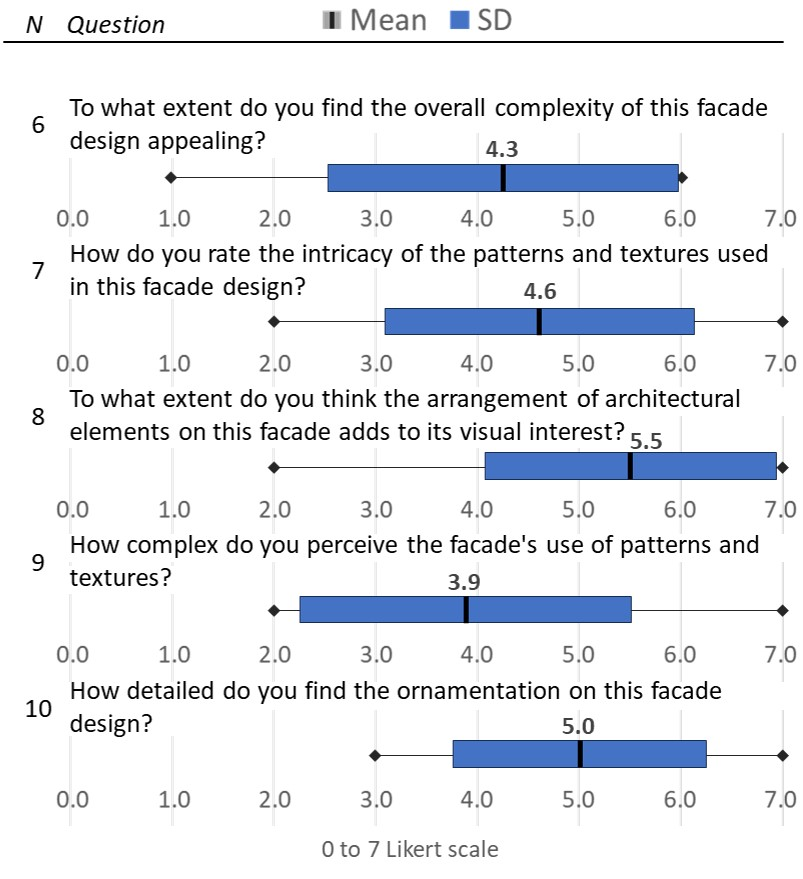
\includegraphics[width=\linewidth]{Images/SurveyPart1Complexity}
        \captionof{figure}{Questions 6 to 10 of the Complexity perception section from the Post-Experiment Survey. \- (n = 10), 1 - strongly disagree, 7 - strongly agree}
        \label{fig:SurveyQuestions6-10} &
        \centering
        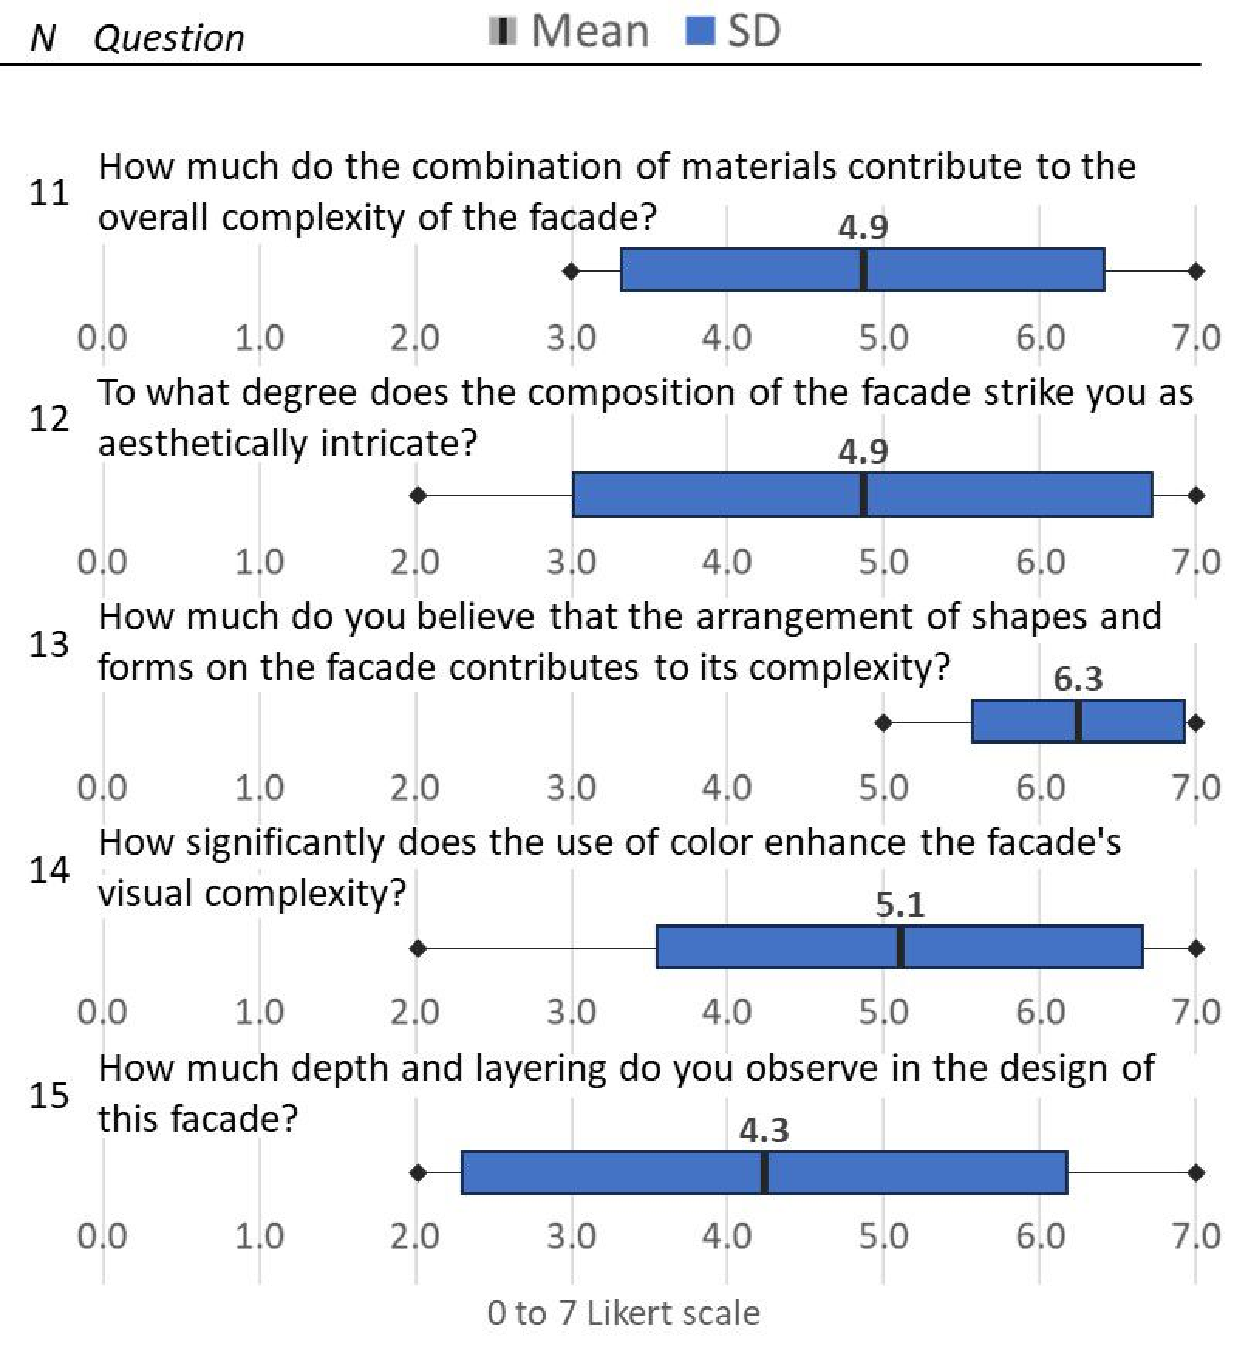
\includegraphics[width=\linewidth]{Images/SurveyPart2Complexity}
        \captionof{figure}{Questions 11 to 15 of the Complexity perception section from the Post-Experiment Survey. \- (n = 10), 1 - strongly disagree, 7 - strongly agree}
        \label{fig:SurveyQuestions11-15}
    \end{tabularx}
\end{table*}


%% Complexity Perception Accuracy Graphs
\begin{table*}[htb]
    \centering
    \small
    \begin{tabularx}{\textwidth}{X X X}
        \centering
        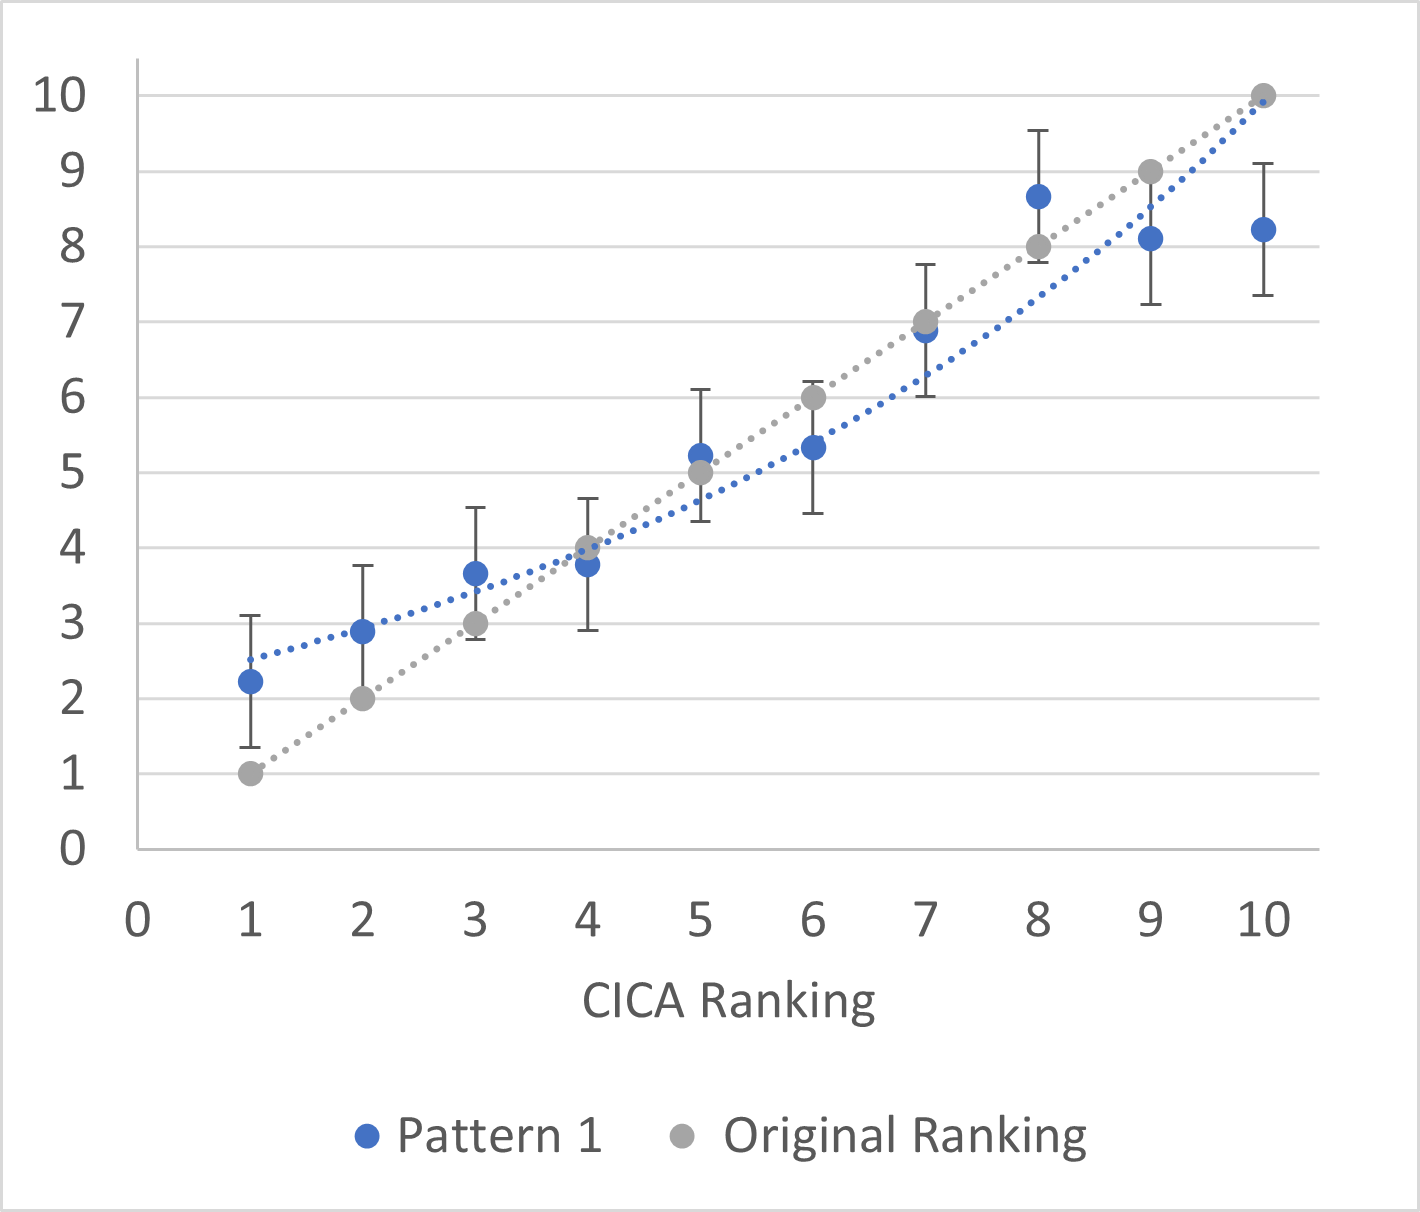
\includegraphics[width=\linewidth]{Images/AccuracyPattern1}
        \captionof{figure}{Accuracy comparison pattern 1 with original ranking}
        \label{fig:AccuracyPattern1} &
        \centering
        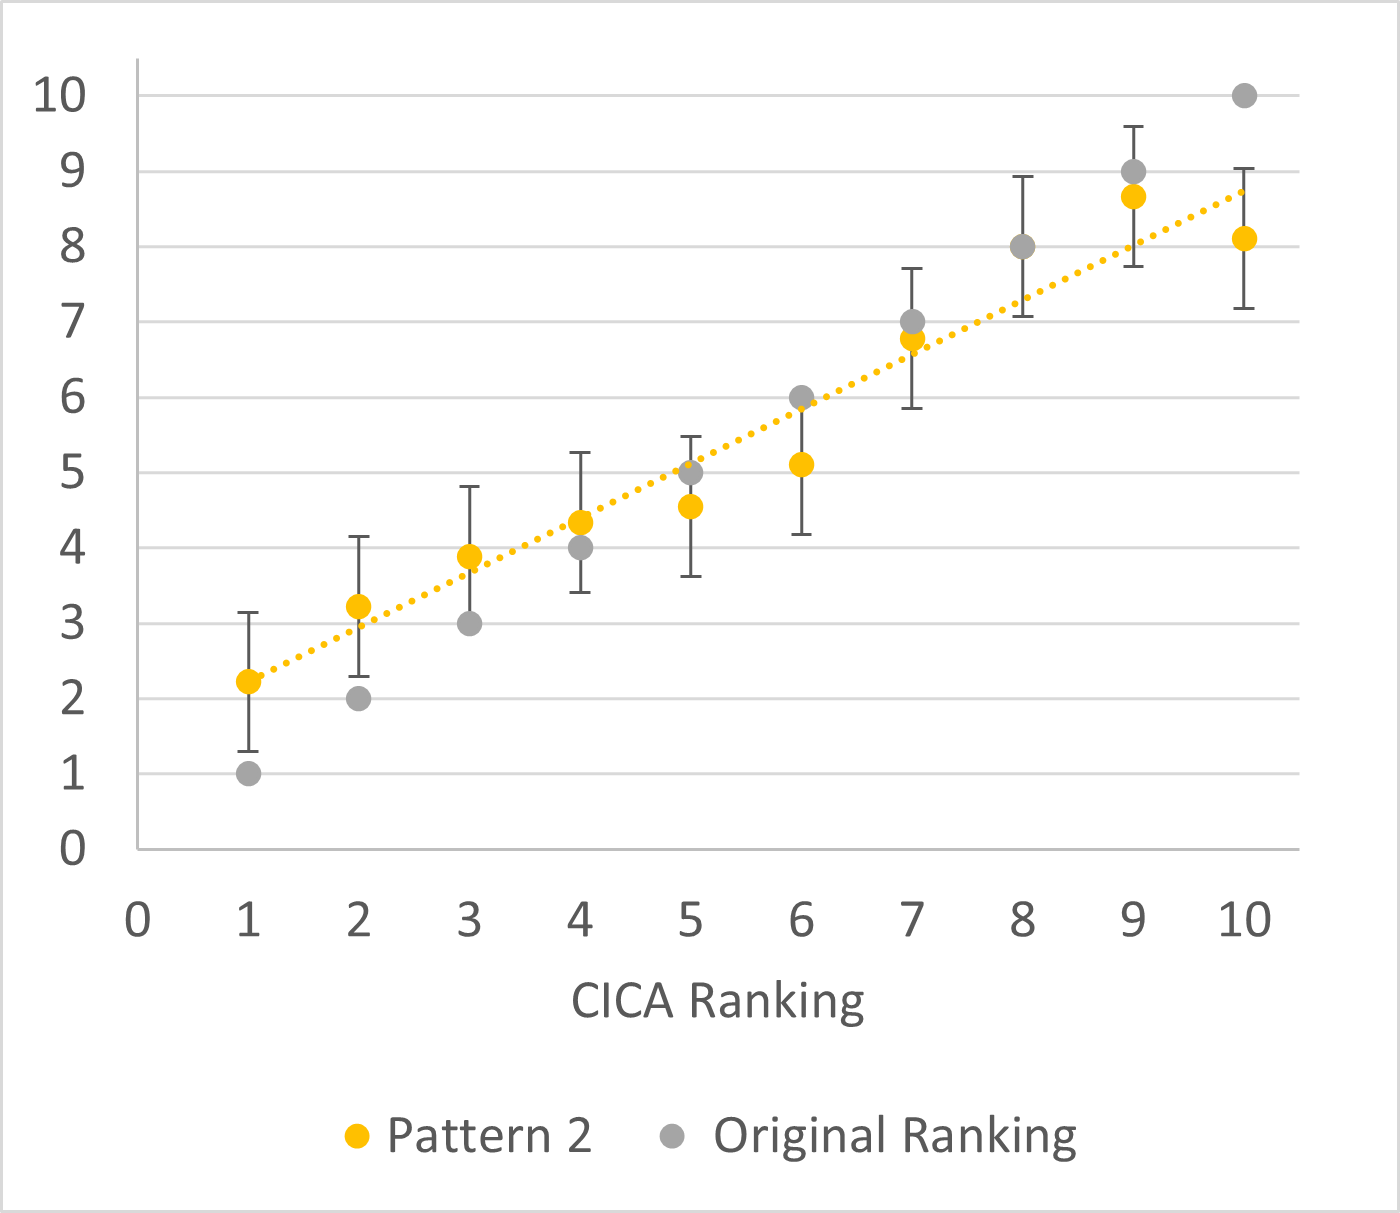
\includegraphics[width=\linewidth]{Images/AccuracyPattern2}
        \captionof{figure}{Accuracy comparison pattern 2 with original ranking}
        \label{fig:AccuracyPattern2} &
        \centering
        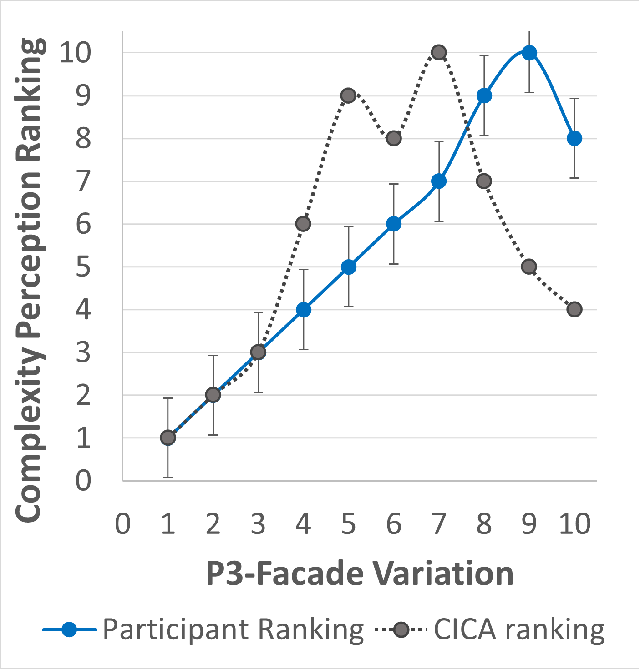
\includegraphics[width=\linewidth]{Images/AccuracyPattern3}
        \captionof{figure}{Accuracy comparison pattern 3 with original ranking}
        \label{fig:AccuracyPattern3}
    \end{tabularx}
\end{table*}

%% Participant background chart and years of experience
\begin{table*}[htb]
        \centering
        \small
        \begin{tabularx}{\textwidth}{X X}
            \centering
            % trim=left 0 down 50 right 0 top 50
            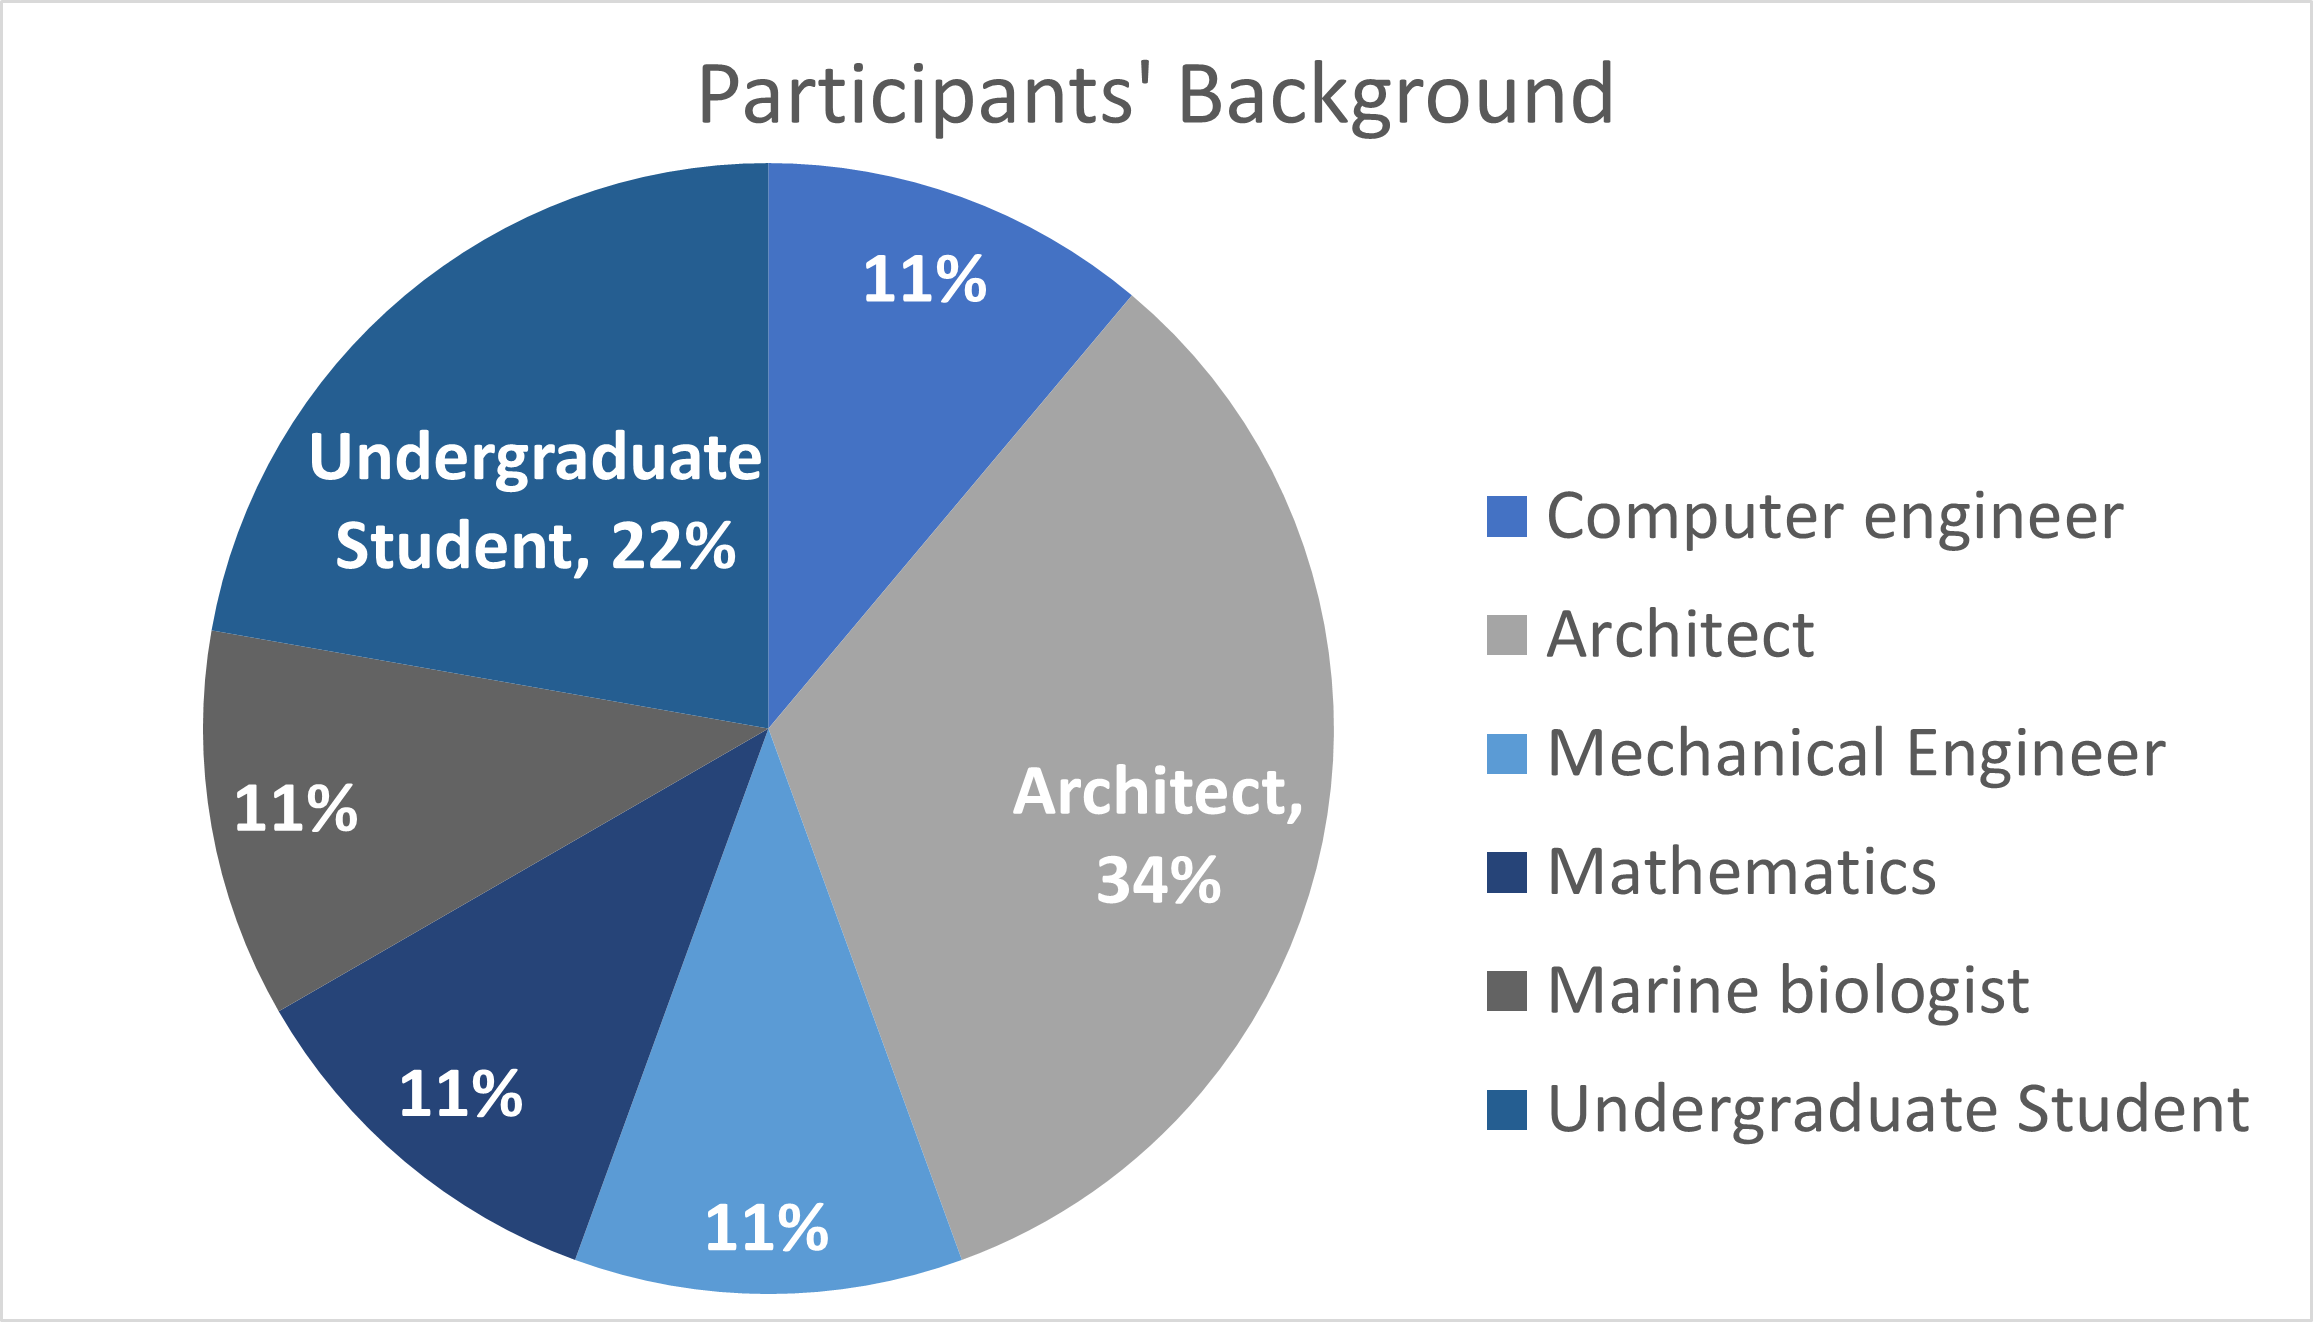
\includegraphics[width=\linewidth, trim=0 60 0 0]{Images/SurveyBackground}
            \captionof{figure}{This chart shows the professional backgrounds of participants involved in the facade design complexity analysis experiment.}
            \label{fig:SurveyBackgroundChart} &
            \centering
            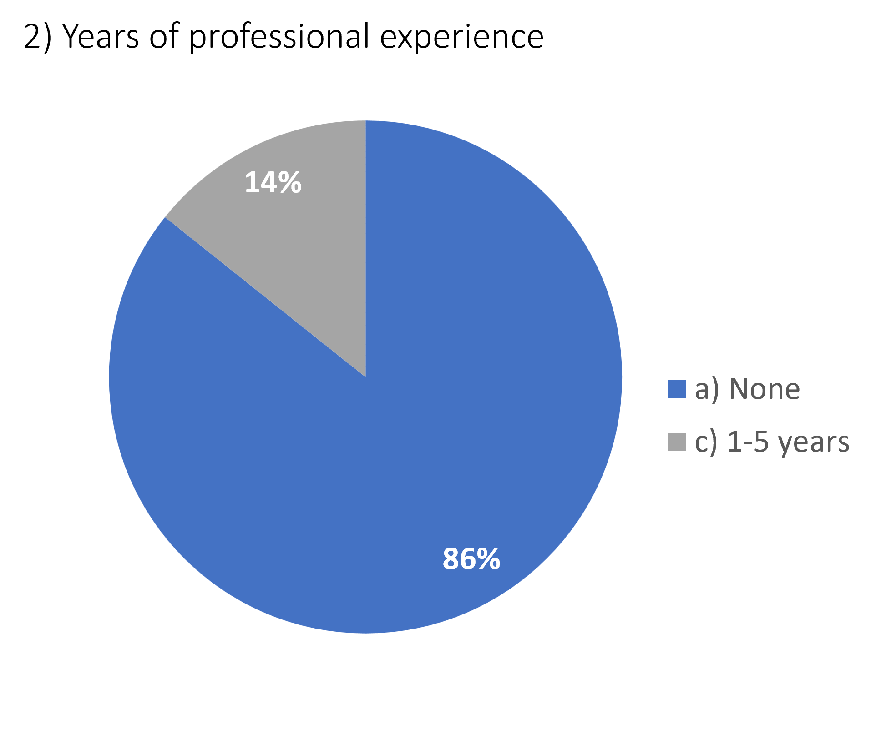
\includegraphics[width=\linewidth, trim=0 60 0 0]{Images/SurveyExperience}
            \captionof{figure}{This chart displays the experience levels in facade design of participants for the study complexity analysis in building design.}
            \label{fig:SurveyYearsExperienceChart}
        \end{tabularx}
    \end{table*}

% Bar Chart of Chosen facade variation for all sessions of the experiment
\begin{figure*}[htb]
    \centering
    %trim=100 180 100 120, clip
    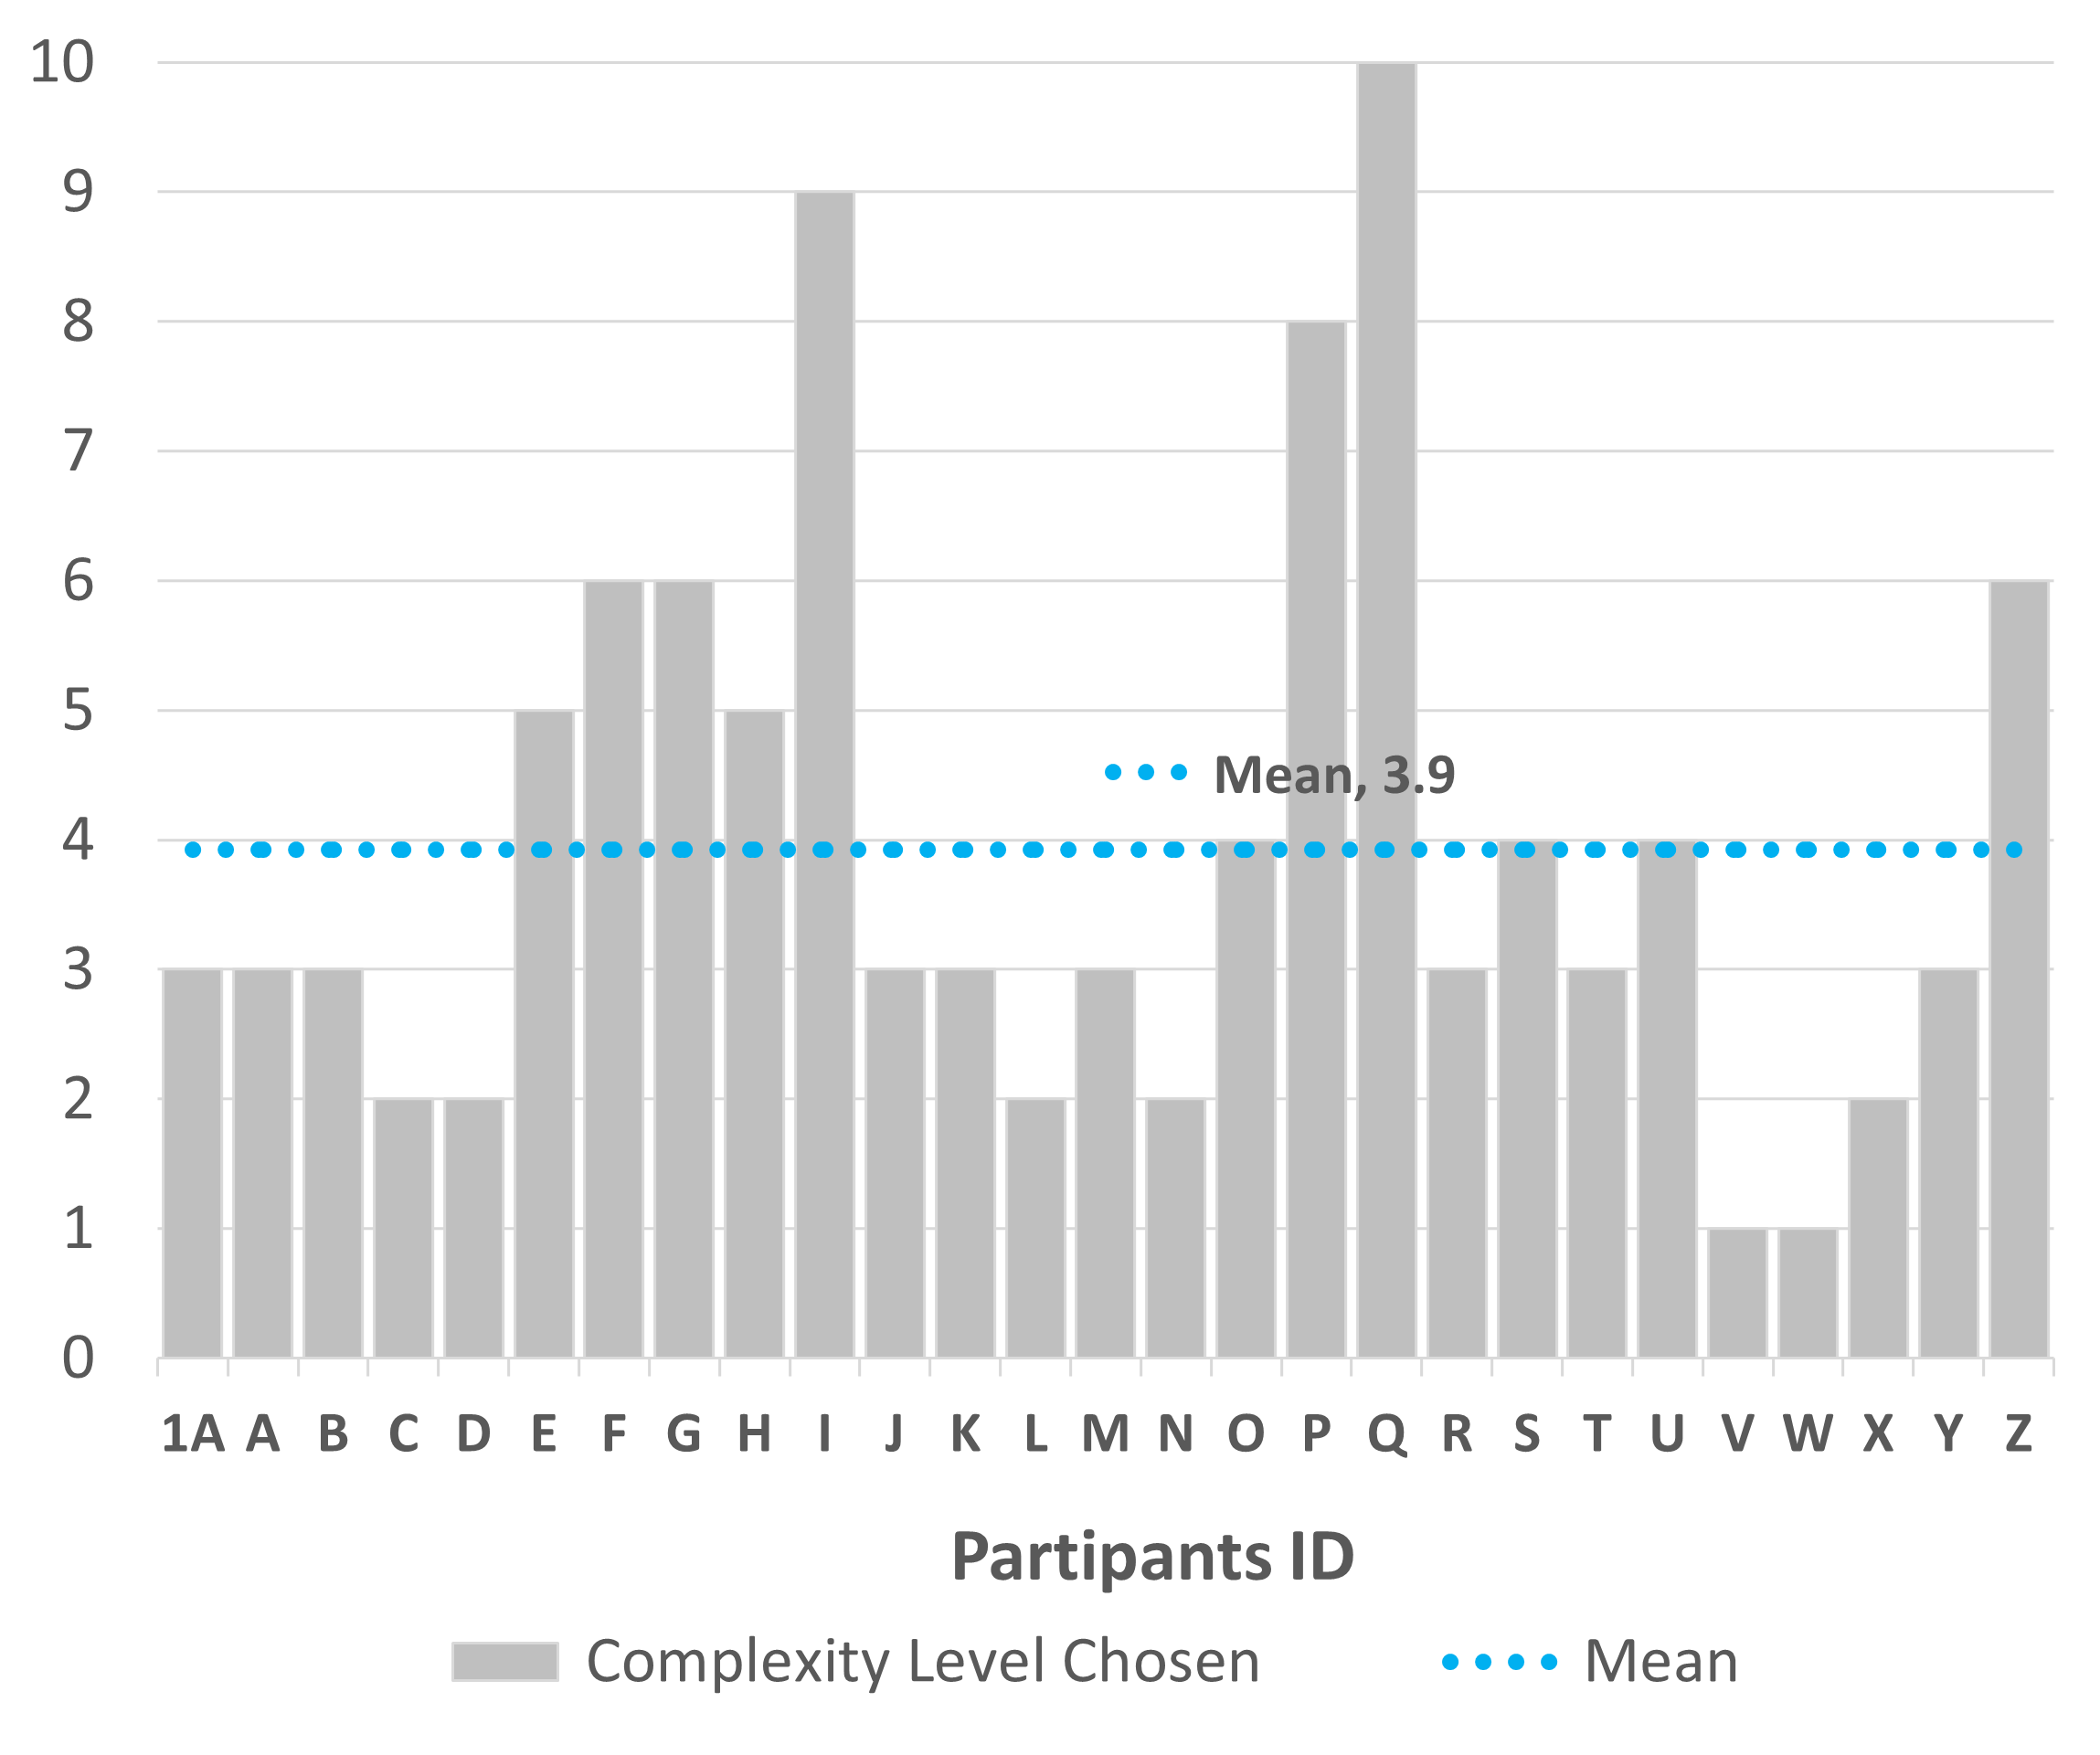
\includegraphics[width=\linewidth]{Images/ComplexityLevelChosenChart}
    \caption{Chart displaying participants' preferred complexity levels among the ten options during the VR simulation stage of the experiment for all three patterns.(CICA Score: Mean = 3.82; SD = 1.1)}
    \label{fig:ComplexityLevelChosenChart}
\end{figure*}

% Probability Chart and Complexity level per Pattern
\begin{table*}[htb]
    \centering
    \small
    \begin{tabularx}{\textwidth}{X X}
        \centering
        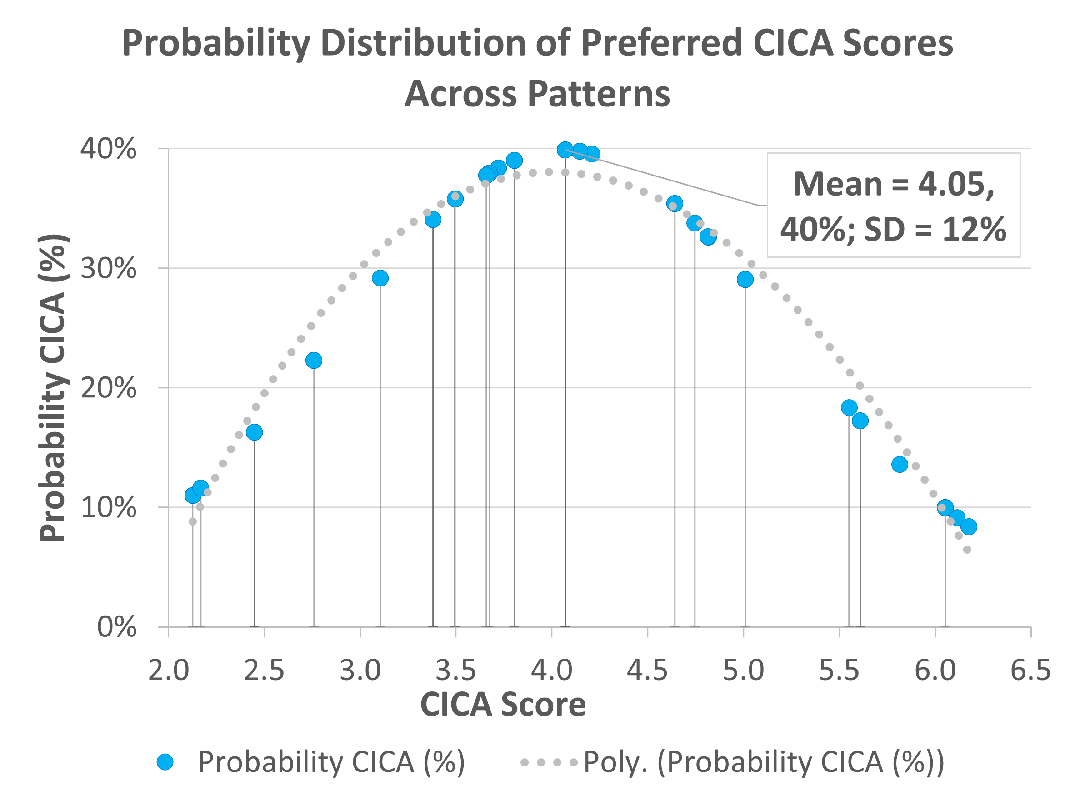
\includegraphics[width=\linewidth]{Images/ProbabilityPreferredComplexitylevel}
        \captionof{figure}{Scatter graph illustrating the probability distribution of preferred CICA score for facade design across all three patterns, derived from data collected during the VR stage of the experiment.(Probability CICA score: \(Mean = 3.82, 40\%\ ; SD = 13\%\))}
        \label{fig:ProbabilityComplexitylevelChart}
        &
        \centering
        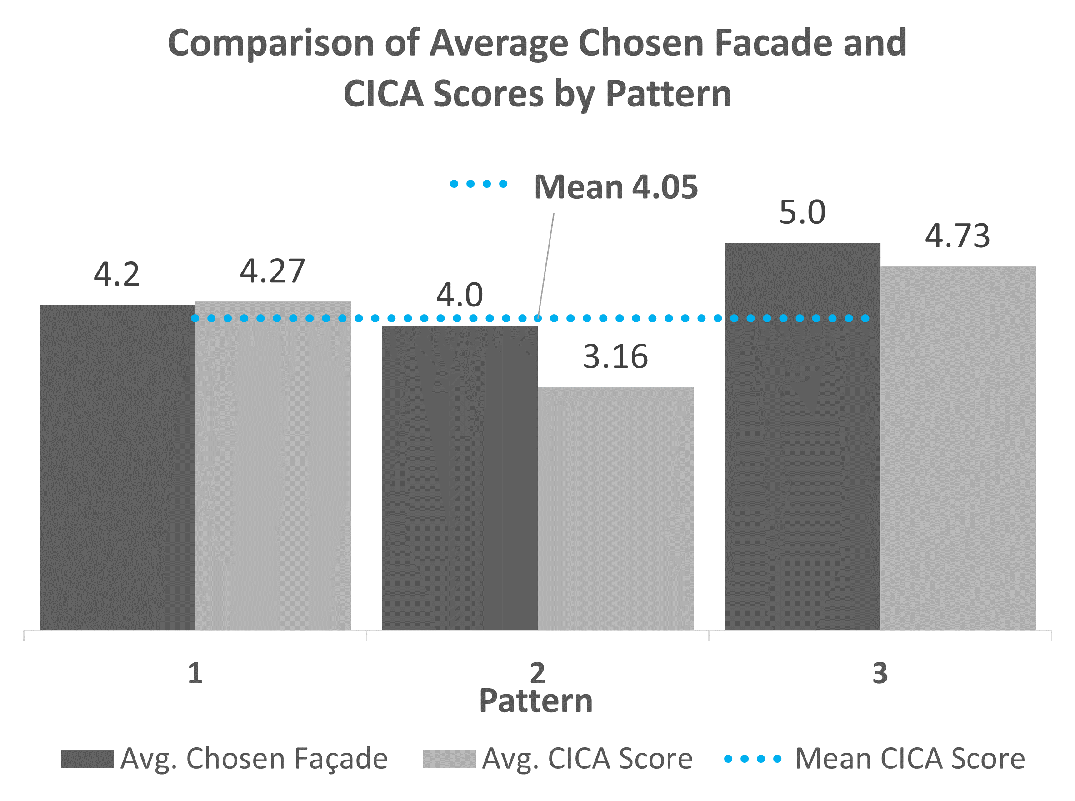
\includegraphics[width=\linewidth]{Images/PreferredComplexityLevelPerPattern}
        \captionof{figure}{Average CICA score of preferred facade variation per pattern chosen by participants during the VR stage of the experiment. (Facade variation: \(Mean = 3.9\). CICA score: \(Mean = 3.82; SD = 1.1\)).}
        \label{fig:ComplexityLevelPerPattern}
    \end{tabularx}
\end{table*}

%f1: Complexity scoring function
\begin{table}[htb]
    \caption{Function 1: Complexity scoring function that integrates various criteria to assess intricacy of a building facade.}
    \label{tab:ComplexityScoreFunction_table}
    \centering
    \small
    \begin{tabular}{|p{8cm}|}
    \hline
        \textbf{\(f_1\), Unified `Complexity Scoring' function 1}\\
        \textit{Calculate the complexity score for all the images on the data pool}
        \\
        \begin{equation}
            f_1(x) = \left[ \mathrm{round}\left(\sum_{i=1}^{n} w_i \cdot a_i, 2\right) \right] = complexity\_score
        \label{eq:F1_ComplexityScoreFunction}
        \end{equation}

        \\
        \textit{ for the Buildings included in the database.}\\
        \\
        \textit{where;} \\
        \\
        \(n \); is the number of performance indicators \\
        \(w_i \); represents the i-th elements weight input and \\
        \(a_i \); represents the i-th normalized score for the respective metric(`Edge Density' and `Contour Count').\\
        \\

        \textit{Finally, the `Complexity score' is assigned to each building for data visualization.}\\
    \hline
    \end{tabular}
\end{table}


%% Figure of Real building next to 3D modeled building
    \begin{figure}[htb]
        \centering
        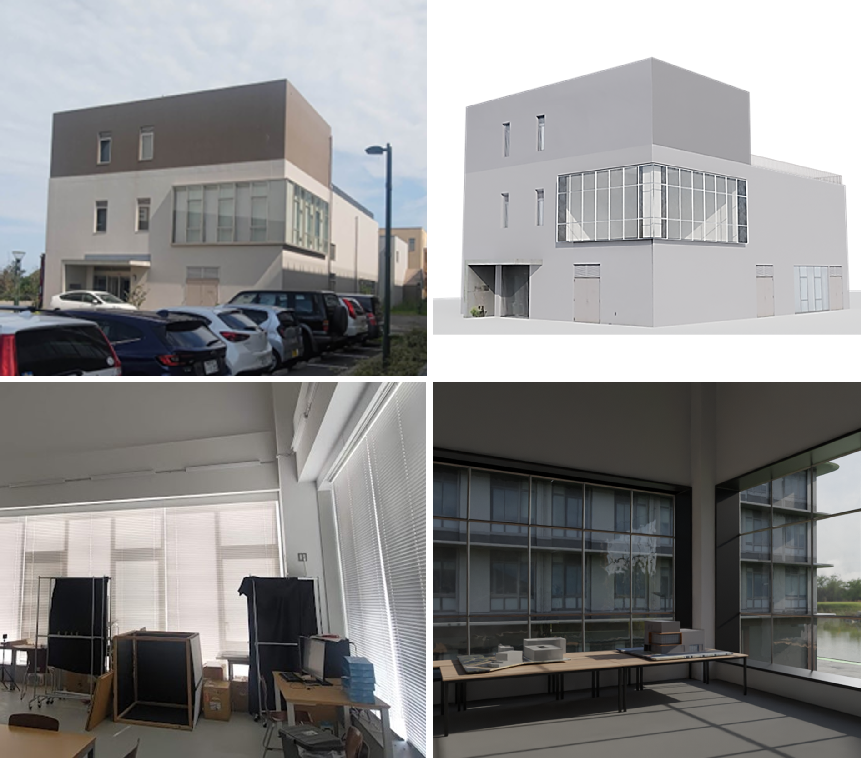
\includegraphics[width= \linewidth]{Images/Realvs3DmodelBlender}
        \caption{Real vs. 3D modeled building for the Facade Design Complexity Analysis experiment.}
        \label{fig:RealVs3dModel}
    \end{figure}

%% Figure of interior and exterior VR
    \begin{figure}[htb]
        \centering
        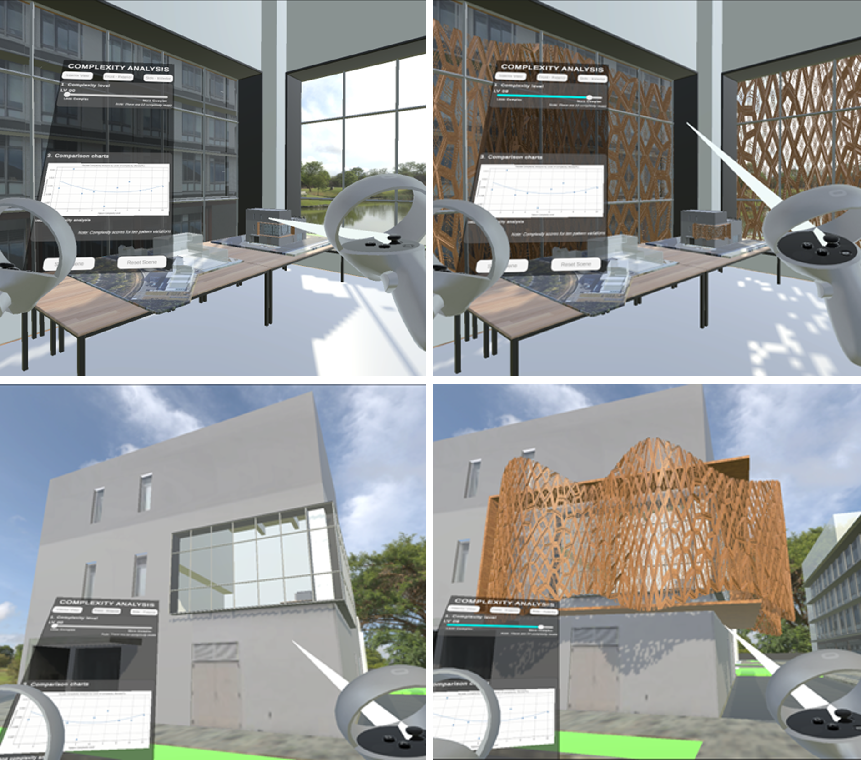
\includegraphics[width= \linewidth]{Images/VRInteriorExterior}
        \caption{Comparison side by side of the VR simulation of interior and exterior of existing laboratory building used for experiment (Left) and VR Simulation of facade variation (Right) used for complexity Analysis.}
        \label{fig:VRInteriorExterior}
    \end{figure}


%% Figure of Old timeline
    \begin{figure*}[htb]
    \centering
    \includegraphics[width= \linewidth]{Images/OldTimeline}
    \caption{Example of historical oscillations between complexity and simplicity in architecture history. (Left to right) Romanesque, Gothic, Classicism, Baroque, Neo-classicism. (\textit{Images edited from source})}
    \label{fig:Oldtimeline}
    \end{figure*}





%!Format for images side by side

\begin{table*}[htb]
    \centering
    \small
    \begin{tabularx}{\textwidth}{X X}
        \centering
        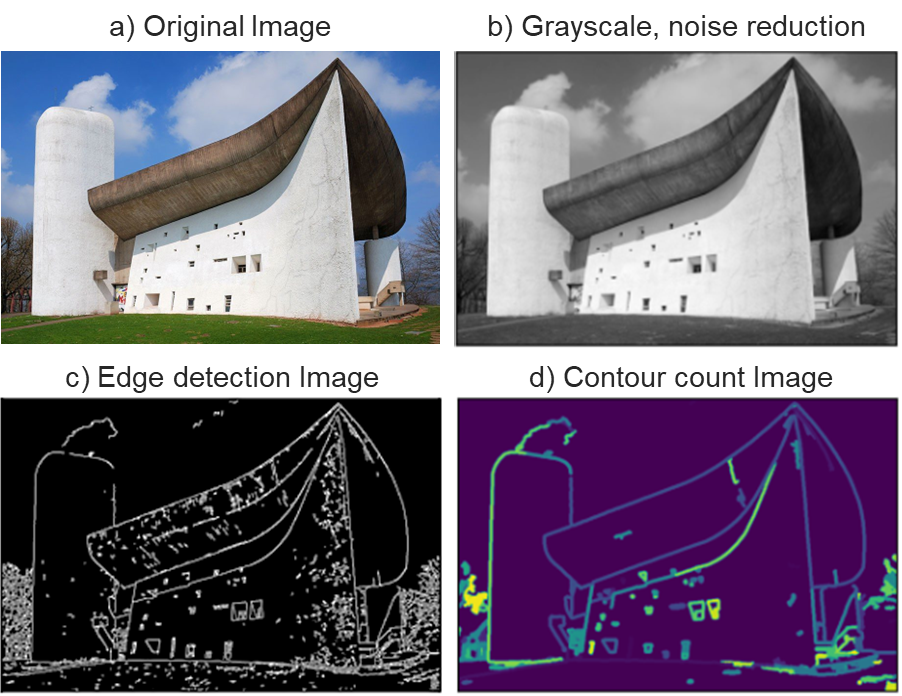
\includegraphics[width= \linewidth]{Images/CICAHistoryPlot}
        \captionof{figure}{Edge Detection analysis of historic buildings demonstrating complexity assessment.}
        \label{fig:ComplexityPlotHistory} &
        \centering
        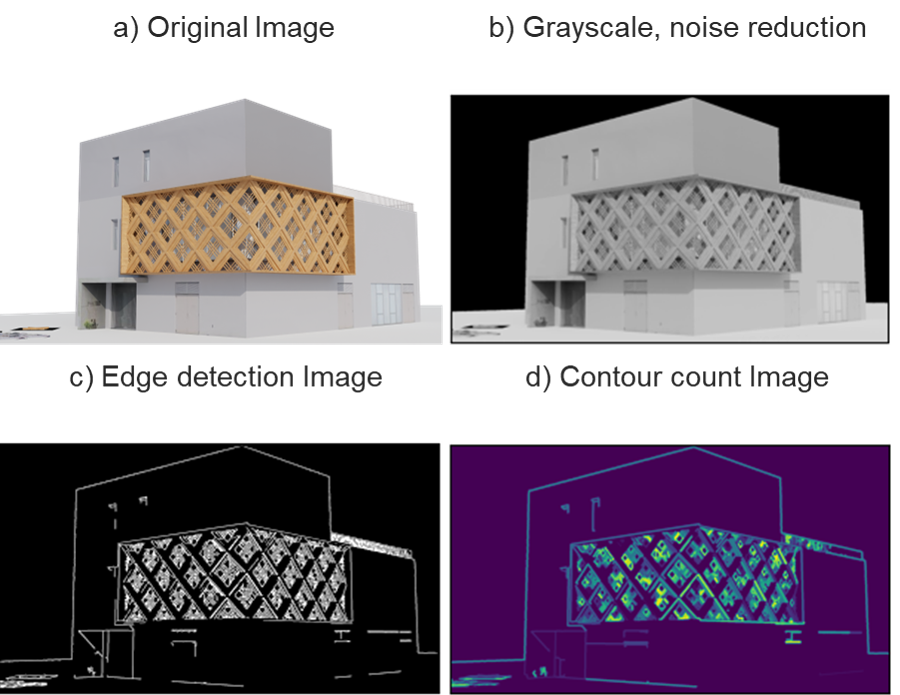
\includegraphics[width= \linewidth]{Images/CICARenderPlot}
        \captionof{figure}{Complexity analysis of 3D-modeled facades for the VR experiment.}
        \label{fig:ComplexityPlotRenderCICA}
        \end{tabularx}
    \end{table*}

%!uNUSED IMAGES
%% Figure Timeline Architecture Image
     \begin{figure}[htb]
          \centering
          % trim=left 190 down 250 right 150 top5
          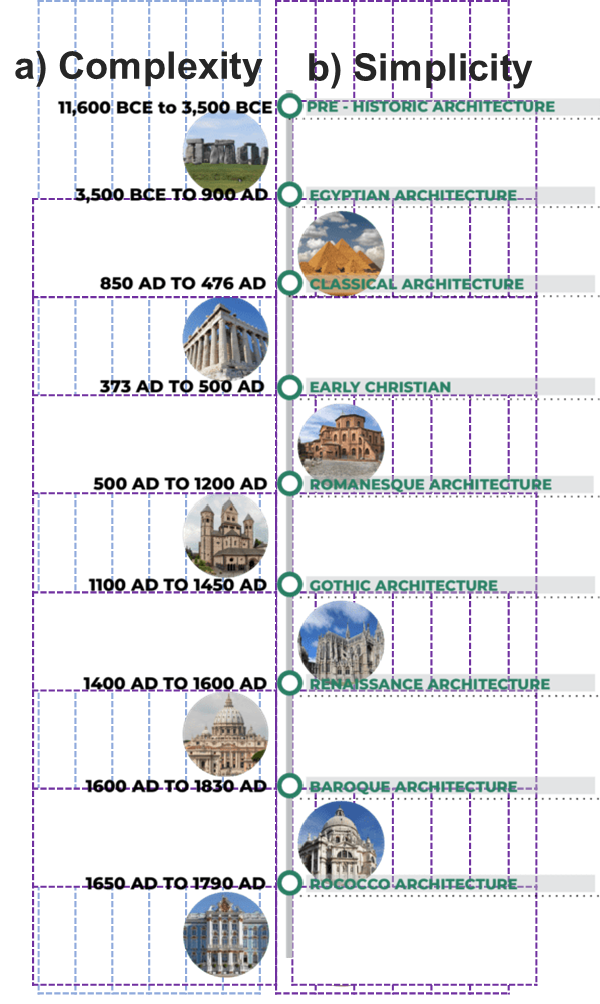
\includegraphics[width= \linewidth]{Images/TimelineArchitecture}
          \caption{Timeline of Architecture and the recurrent pattern of complexity and simplicity}
          \label{fig:TimelineArchitecture}
        \end{figure}

%%Figure Romanesque vs Gothic figure
     \begin{figure}[htb]
          \centering
          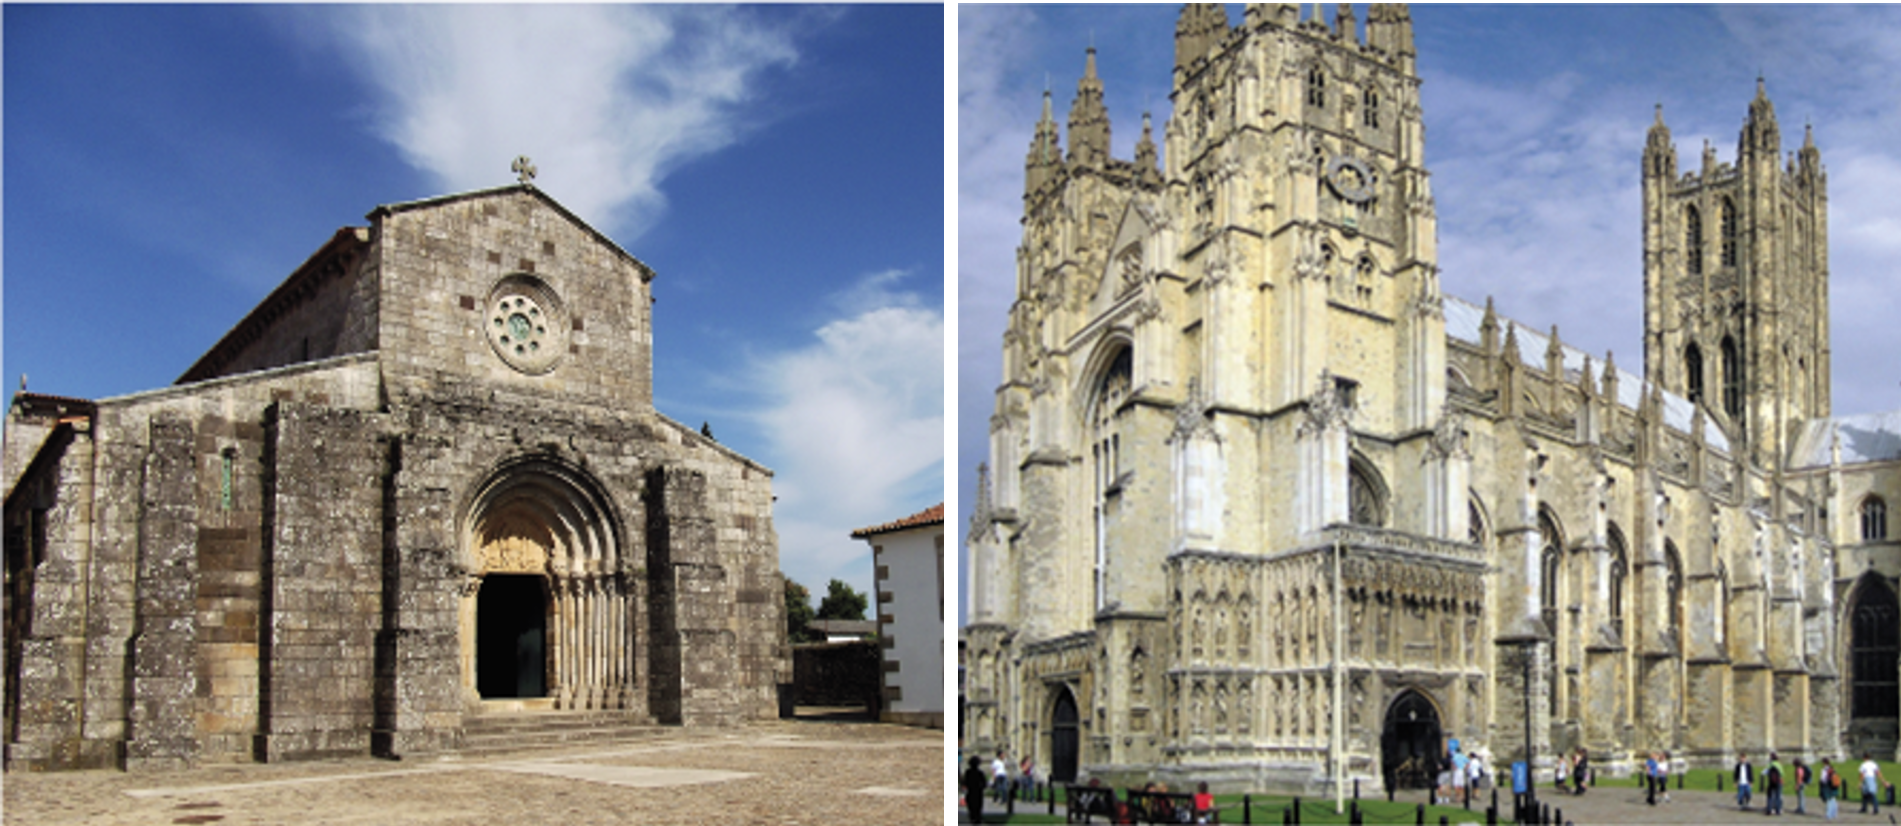
\includegraphics[width= \linewidth]{Images/RomanesqueVsGothic}
          \caption{Romanesque Church 10th AC (left) vs Gothic church 12th AC (right). From simplicity to complexity. (\textit{Images edited from source})}
          \label{fig:RomanesquevsGothic}
        \end{figure}

%%Figure ArtNouvau vs Modernism
     \begin{figure}[htb]
          \centering
          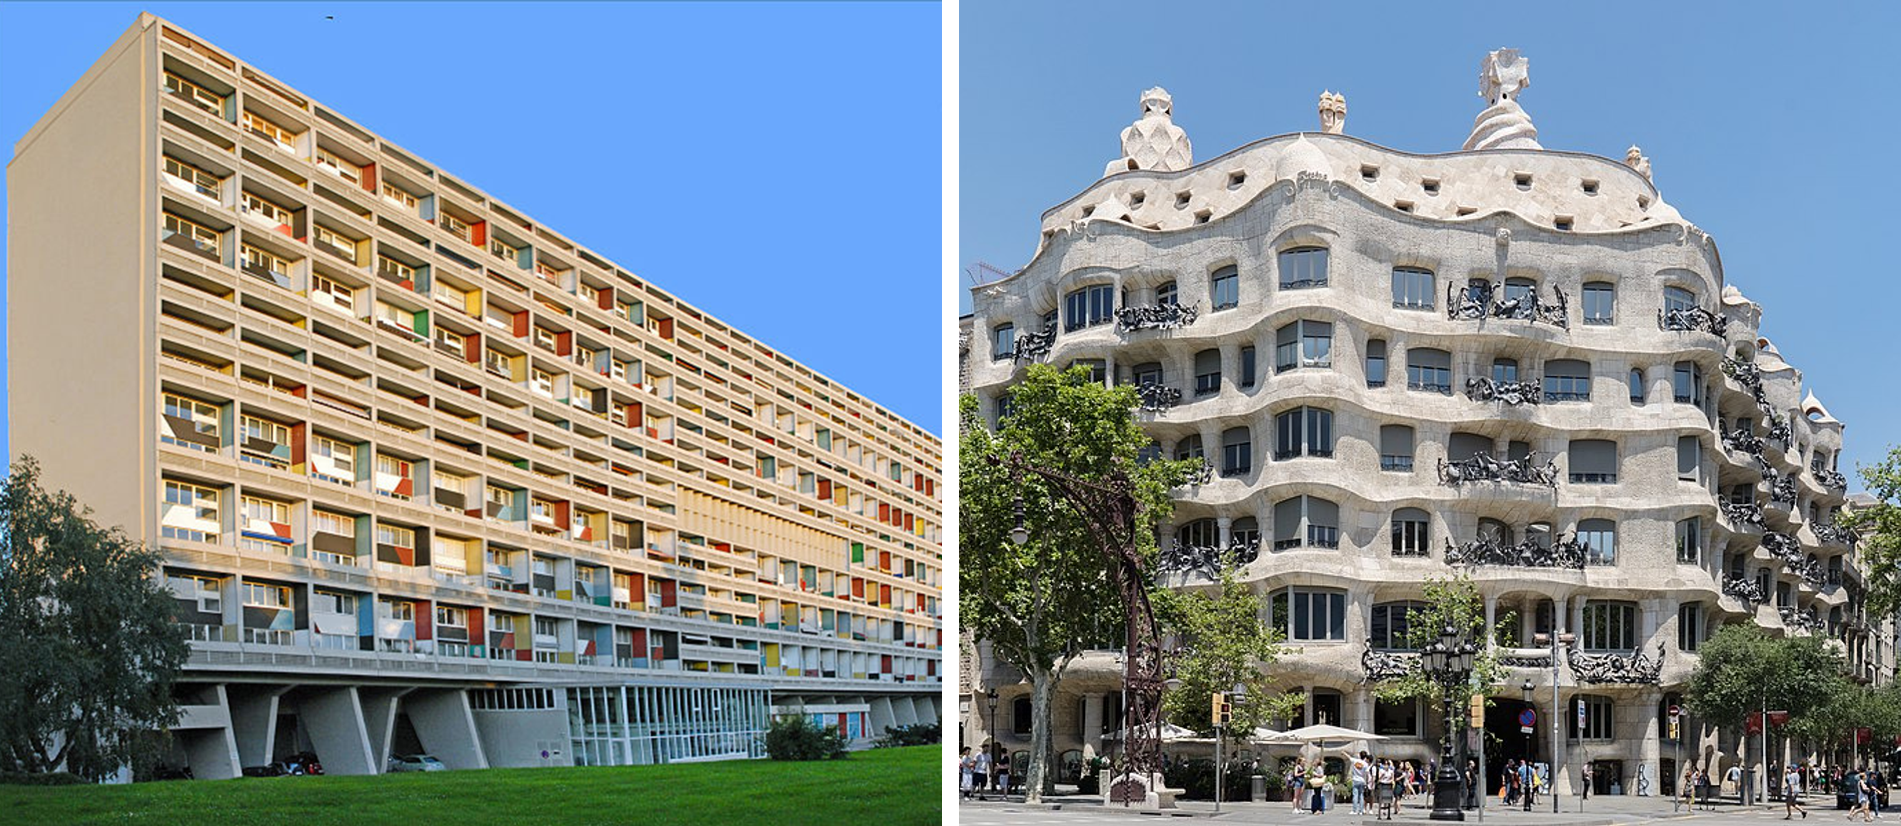
\includegraphics[width= \linewidth]{Images/ArtNouveauVsModernism}
          \caption{Modern Architecture 20th century (Left) vs Art Nouveau building 1920's 30's (Right). To simplicity from complexity. (\textit{Images edited from source})}
          \label{fig:ArtNouveauVsModernism}
        \end{figure}

%%Figure Modernism vs contemporary
     \begin{figure}[htb]
          \centering
          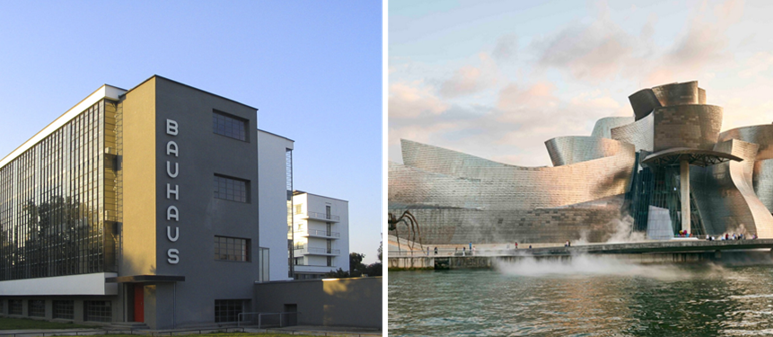
\includegraphics[width= \linewidth]{Images/modernism vs postmodernism}
          \caption{Modernist building "Bauhaus School" 20th AC (left) vs Postmodernist "Guggenheim museum" 1997 (right). From simplicity to Complexity. (\textit{Images edited from source:\cite{Arora2023}})}
          \label{fig:Modernismvscontemporary}
        \end{figure}

%%Figure neoclassicim vs modernism
     \begin{figure}[htb]
          \centering
          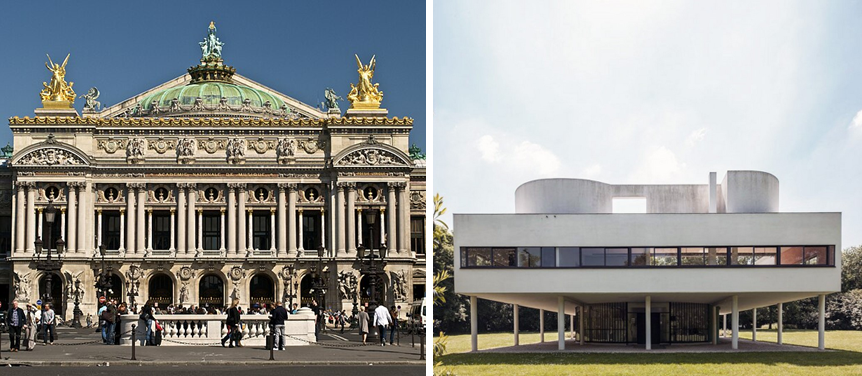
\includegraphics[width= \linewidth]{Images/NeoclassicismVsModernism}
          \caption{Neoclassic building "Paris Opera" 19th AC (left) vs Modernist house "Villa Savoye" 20th AC (right). From Complexity to simplicity. (\textit{Images edited from source:\cite{Stacbond2020}})}
          \label{fig:NeoclassicalvsModernism}
        \end{figure}

    %% Figure of baroque facade vs contemporary facade
    \begin{figure}[htb]
        \centering
        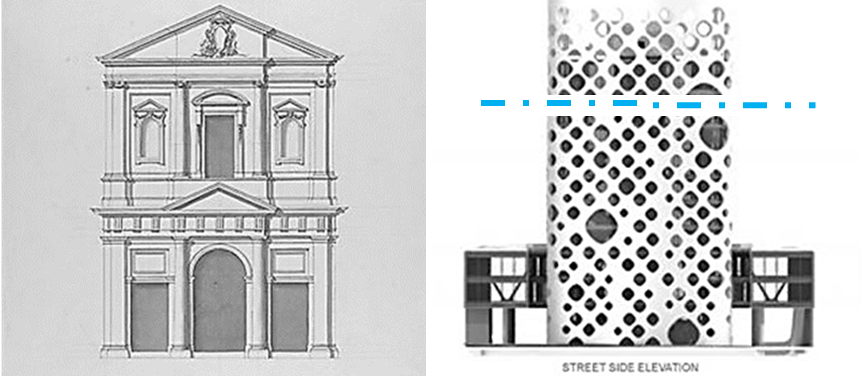
\includegraphics[width= \linewidth]{Images/BaroqueVsContemporaryfacade}
        \caption{Evolution of facade design.
        Baroque Facade 1639 by Bernini (left) vs Contemporary facade, building O-14 by Reiser + Umemoto, 21st Century (right). (\textit{Images edited from source})}
        \label{fig:FacadeBaroqueVsContemporary}
    \end{figure}

    %% Figure of Vitruvian Architecture
    \begin{figure}[htb]
    \centering
    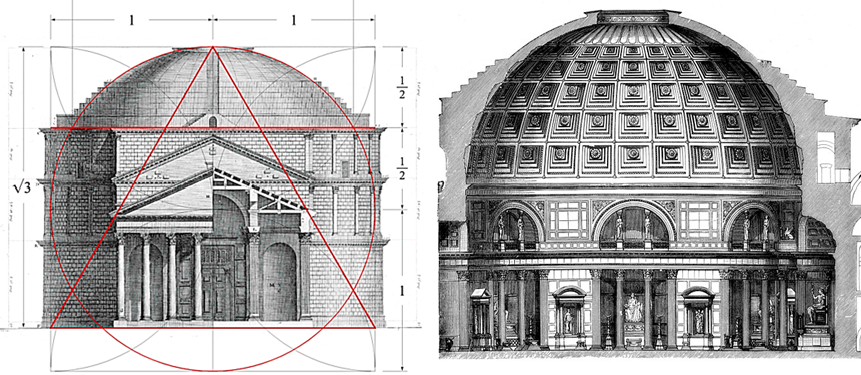
\includegraphics[width= \linewidth]{Images/VitruvianArchitecture}
    \caption{Facade and ornament according to Vitruvius, with emphasis on order, symmetry, and harmony. Pantheon's facade (left) and cross-section (right) symmetry analysis. (\textit{Images edited from source})}
    \label{fig:Vitruvianarchitecture}
    \end{figure}

    %% Figure of Baroque facade Borromini
    \begin{figure}[htb]
    \centering
    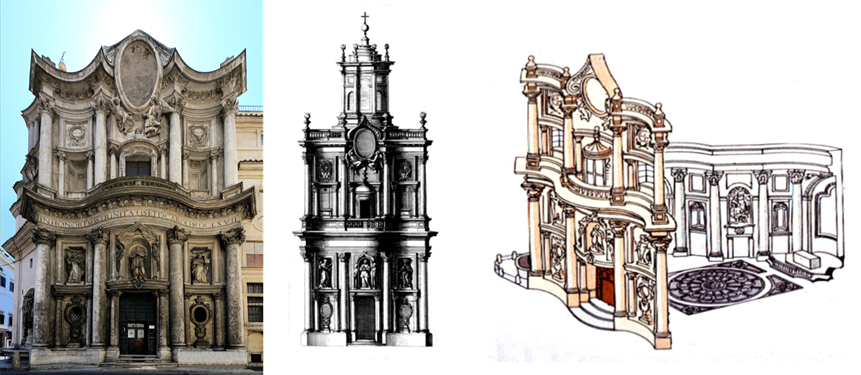
\includegraphics[width= \linewidth]{Images/BaroquefacadeBorromini}
    \caption{Borromini's Interpretation of Facade and Ornament: Elaborate geometric patterns, curved forms, and sculptural elements reflecting internal spatial arrangements. Analysis of San Carlo alle Quattro Fontane Church Facade (left) and Cross Section (right) from its construction in the 1630s, Rome. (\textit{Images edited from source})}
    \label{fig:BorrominiArchitecture}
    \end{figure}

    %% Figure of Classicism and Neo-Classicism facade
    \begin{figure}[htb]
    \centering
    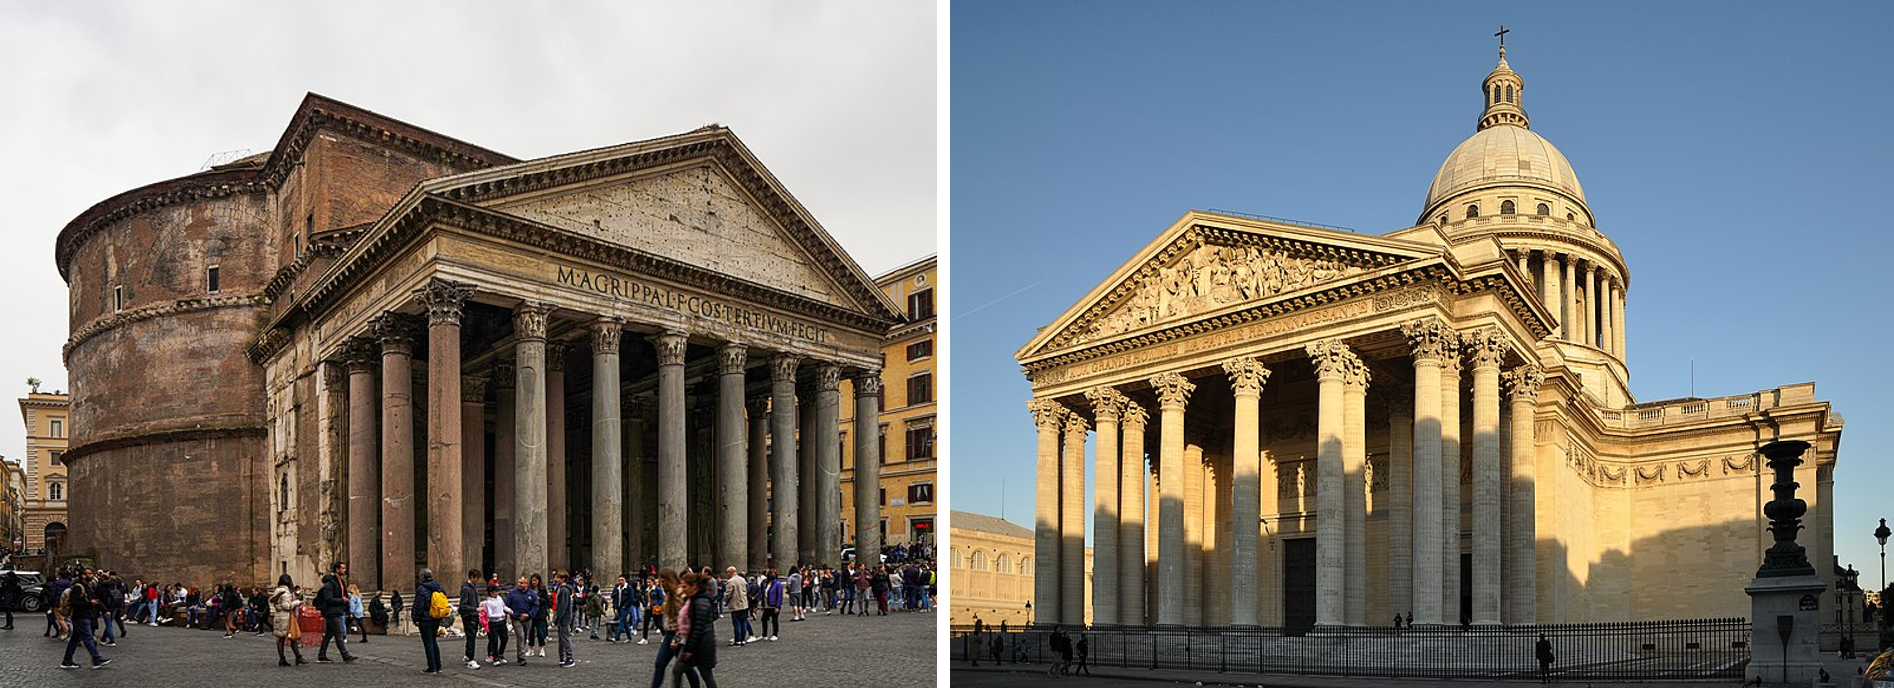
\includegraphics[width= \linewidth]{Images/ClassicismNeoClassicism}
    \caption{Neo-Classical Facades: Emphasis on formal elegance and symmetry. (Left) Pantheon in Rome, 27 BC. (Right) Pantheon in Paris, 1758-1790, Neoclassical style. (\textit{Images edited from source})}
    \label{fig:ClassicismNeoClassicism}
    \end{figure}

    %% Figure of Art Nouveau style facade
    \begin{figure}[htb]
    \centering
    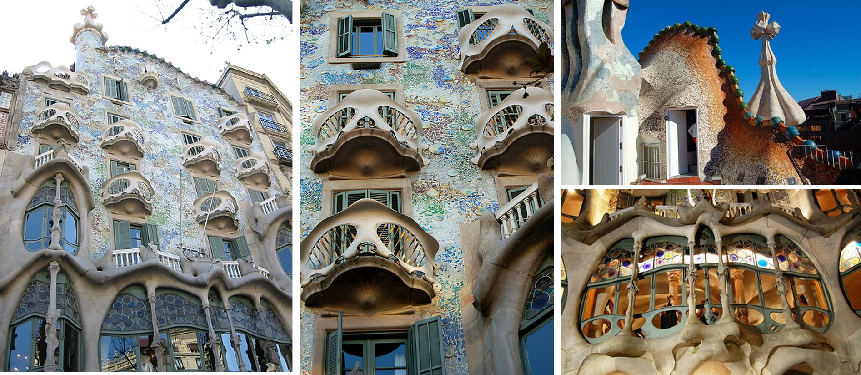
\includegraphics[width= \linewidth]{Images/ArtnouveauGaudi}
    \caption{Art Nouveau Style: Organic forms and nature-inspired motifs. Casa Batlló by Gaudi, 1904. (\textit{Images edited from source})}
    \label{fig:ArtNouveaustyle}
    \end{figure}

    %% Figure of Art Deco style facade
    \begin{figure}[htb]
    \centering
    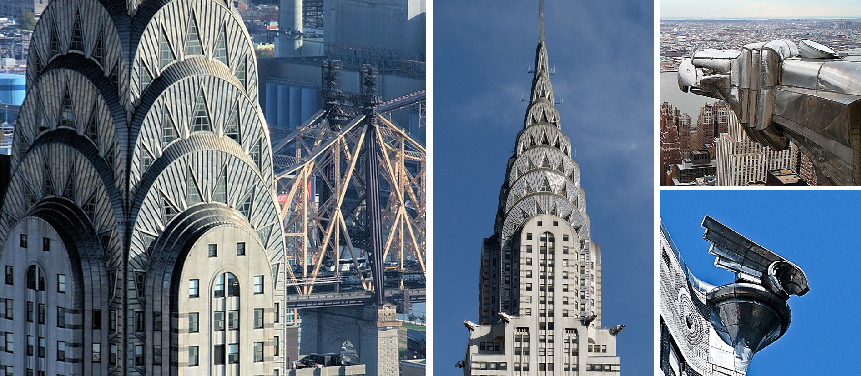
\includegraphics[width= \linewidth]{Images/ArtDecoFacade}
    \caption{Art Deco: Fusion of modernity and historical nostalgia. Chrysler Building, 1930. (\textit{Images edited from source})}
    \label{fig:ArtDeco}
    \end{figure}

    %% Figure of Art Nouveau style facade
    \begin{figure}[hb]
    \centering
    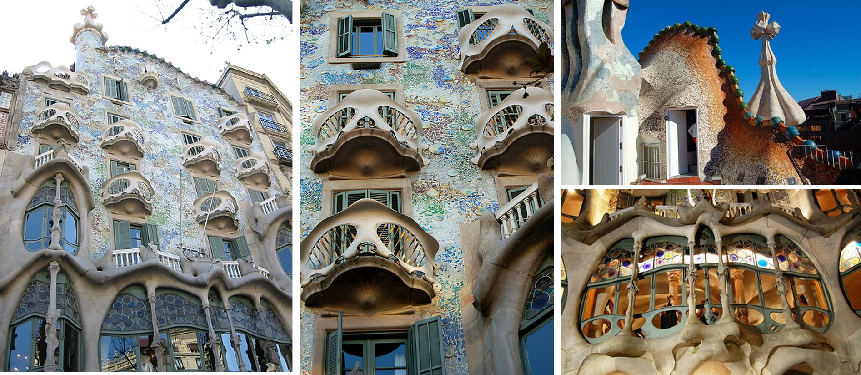
\includegraphics[width= \linewidth]{Images/ArtnouveauGaudi}
    \caption{Art Nouveau Style: Organic forms and nature-inspired motifs. Casa Batlló by Gaudi, 1904. (\textit{Images edited from source})}
    \label{fig:ArtNouveaustyle}
    \end{figure}

    %% Figure of Art Deco style facade
    \begin{figure}[hb]
    \centering
    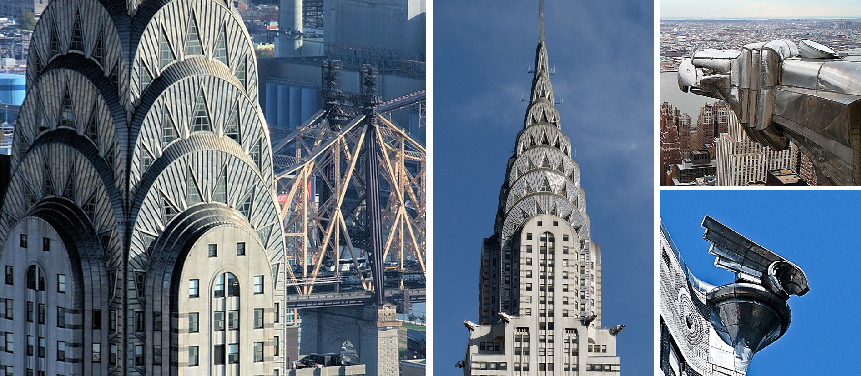
\includegraphics[width= \linewidth]{Images/ArtDecoFacade}
    \caption{Art Deco: Fusion of modernity and historical nostalgia. Chrysler Building, 1930. (\textit{Images edited from source})}
    \label{fig:ArtDeco}
    \end{figure}

    %% Figure of Modernist facade and ornament by Le Corbusier
    \begin{figure}[htb]
        \centering
        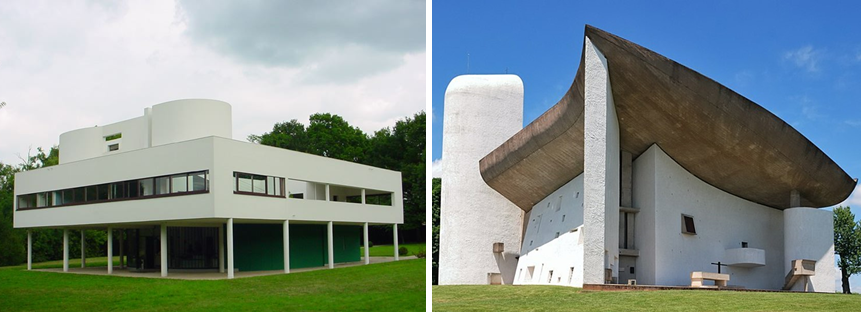
\includegraphics[width= \linewidth]{Images/ModernistFacade}
        \caption{Functionalism in Modernist Facade Design: Le Corbusier's approach. (Left) Villa Savoye, 1928--1931. (Right) Chapelle Notre-Dame-du-Haut de Ronchamp, 1955. (\textit{Images edited from source})}
        \label{fig:Modernistfacade}
    \end{figure}

    %% Figure of Postmodernism ornament
    \begin{figure}[htb]
        \centering
        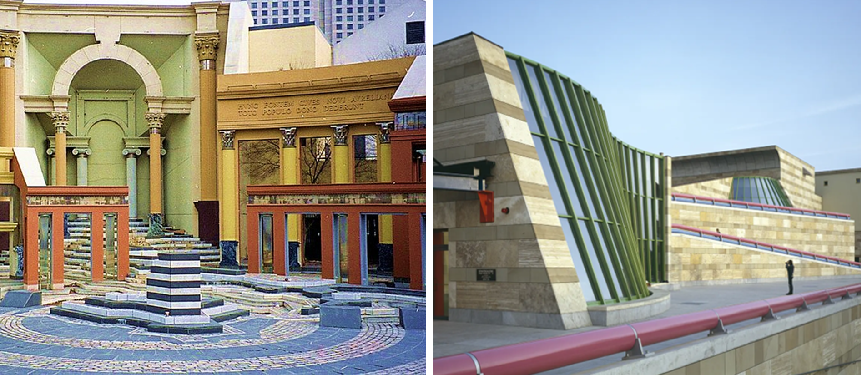
\includegraphics[width= \linewidth]{Images/PostmodernOrnament}
        \caption{Postmodernism's Diverse Ornamentation: (Left) Piazza d’Italia, 1978. (Right) Neue Staatsgalerie, 1984. (\textit{Images edited from source})}
        \label{fig:postmodernOrnamnet}
    \end{figure}

    %% Figure of Old timeline
    \begin{figure*}[htb]
    \centering
    \includegraphics[width= \linewidth]{Images/OldTimeline}
    \caption{Example of historical oscillations between complexity and simplicity in architecture history. (Left to right) Romanesque, Gothic, Classicism, Baroque, Neo-classicism. (\textit{Images edited from source})}
    \label{fig:Oldtimeline}
    \end{figure*}

    %% Figure of Middle timeline
    \begin{figure*}[htb]
    \centering
    \includegraphics[width= \linewidth]{Images/MiddleTimeline}
    \caption{Example of historical oscillations between complexity and simplicity in architecture history. (Left to right) Art Nouveau, Art Deco, Modernism, Post Modernism. (\textit{Images edited from source})}
    \label{fig:Middletimeline}
    \end{figure*}

    %% Figure of Contemporary timeline
    \begin{figure*}[htb]
    \centering
    \includegraphics[width= \linewidth]{Images/contemporaryTimeline}
    \caption{Era of exploration in contemporary architecture. (Left to right) Deconstructivism, Neofuturism, High-tech modernism, Parametricism, Pragmatic utopianism. (\textit{Images edited from source})}
    \label{fig:contemporarytimeline}
    \end{figure*}

    %%Figure Canny Edge of historic buildings
    \begin{figure}[htb]
    \centering
    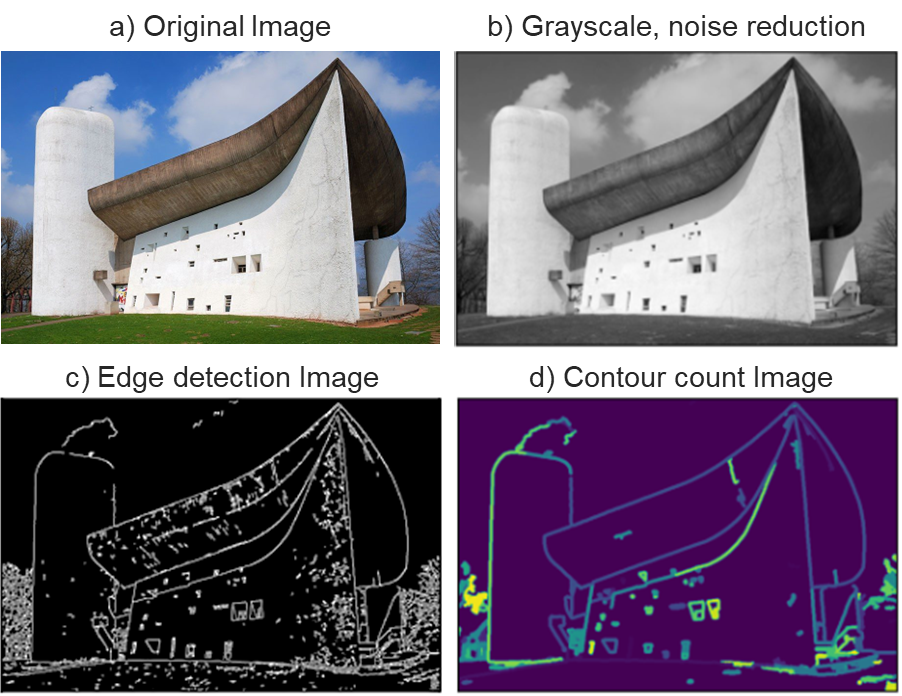
\includegraphics[width= \linewidth]{Images/CICAHistoryPlot}
    \caption{Edge Detection analysis of historic buildings demonstrating complexity assessment.}
    \label{fig:ComplexityPlotHistory}
    \end{figure}


    %%Figure Canny Edge of render buildings
    \begin{figure}[htb]
    \centering
    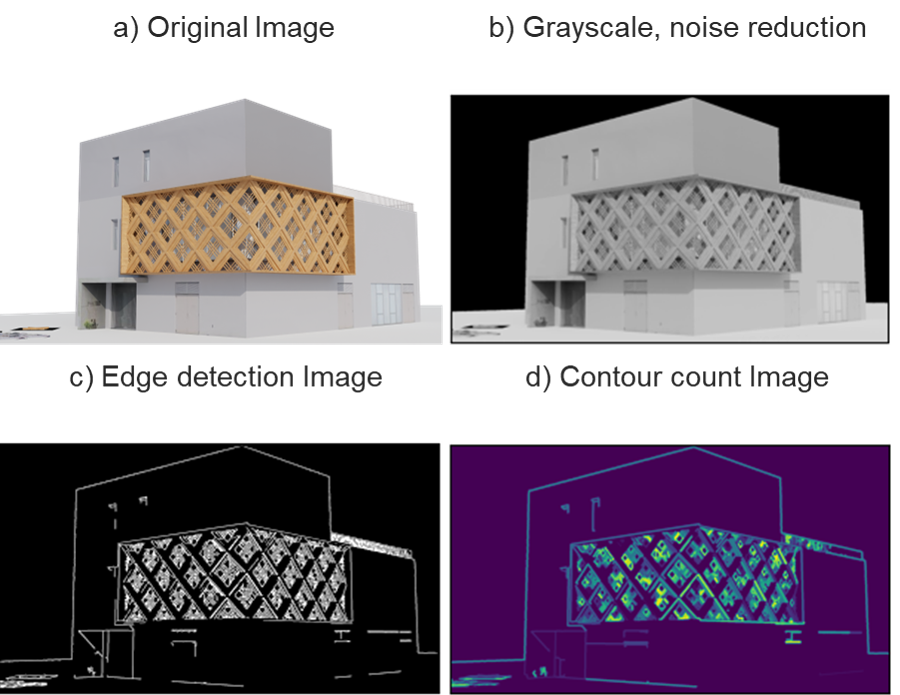
\includegraphics[width= \linewidth]{Images/CICARenderPlot}
    \caption{Complexity analysis of 3D-modeled facades for the VR experiment.}
    \label{fig:ComplexityPlotRenderCICA}
    \end{figure}

%% Figure of Postmodernism facade and ornament
\begin{figure}[htb]
\centering
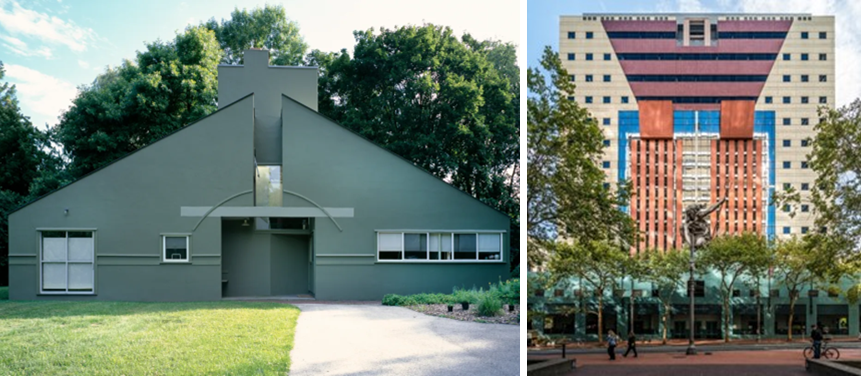
\includegraphics[width= \linewidth]{Images/PostmodernismVenturi}
\caption{Postmodernism's Complexity and Contradiction: (Left) Vanna Venturi House, 1964. (Right) Portland Municipal Services Building, 1982. (\textit{Images edited from source})}
\label{fig:postmodernfacade}
\end{figure}

Similarly, the elaborate Art Deco architecture of the 1920s stands in stark contrast to the subsequent embrace of simplicity of Modern Architecture and rationalism  of the mid-20th century that championed functionalism and minimalist aesthetics, showcasing innovative materials like steel, glass, and concrete\cite{Stacbond2020}(see Figure\ref{fig:ArtNouveauVsModernism}).



%! Original alternative for accuracy graphs alternative


 %% Figure Complexity perception per level with trendlines
    \begin{figure*}[htb]
      \centering
      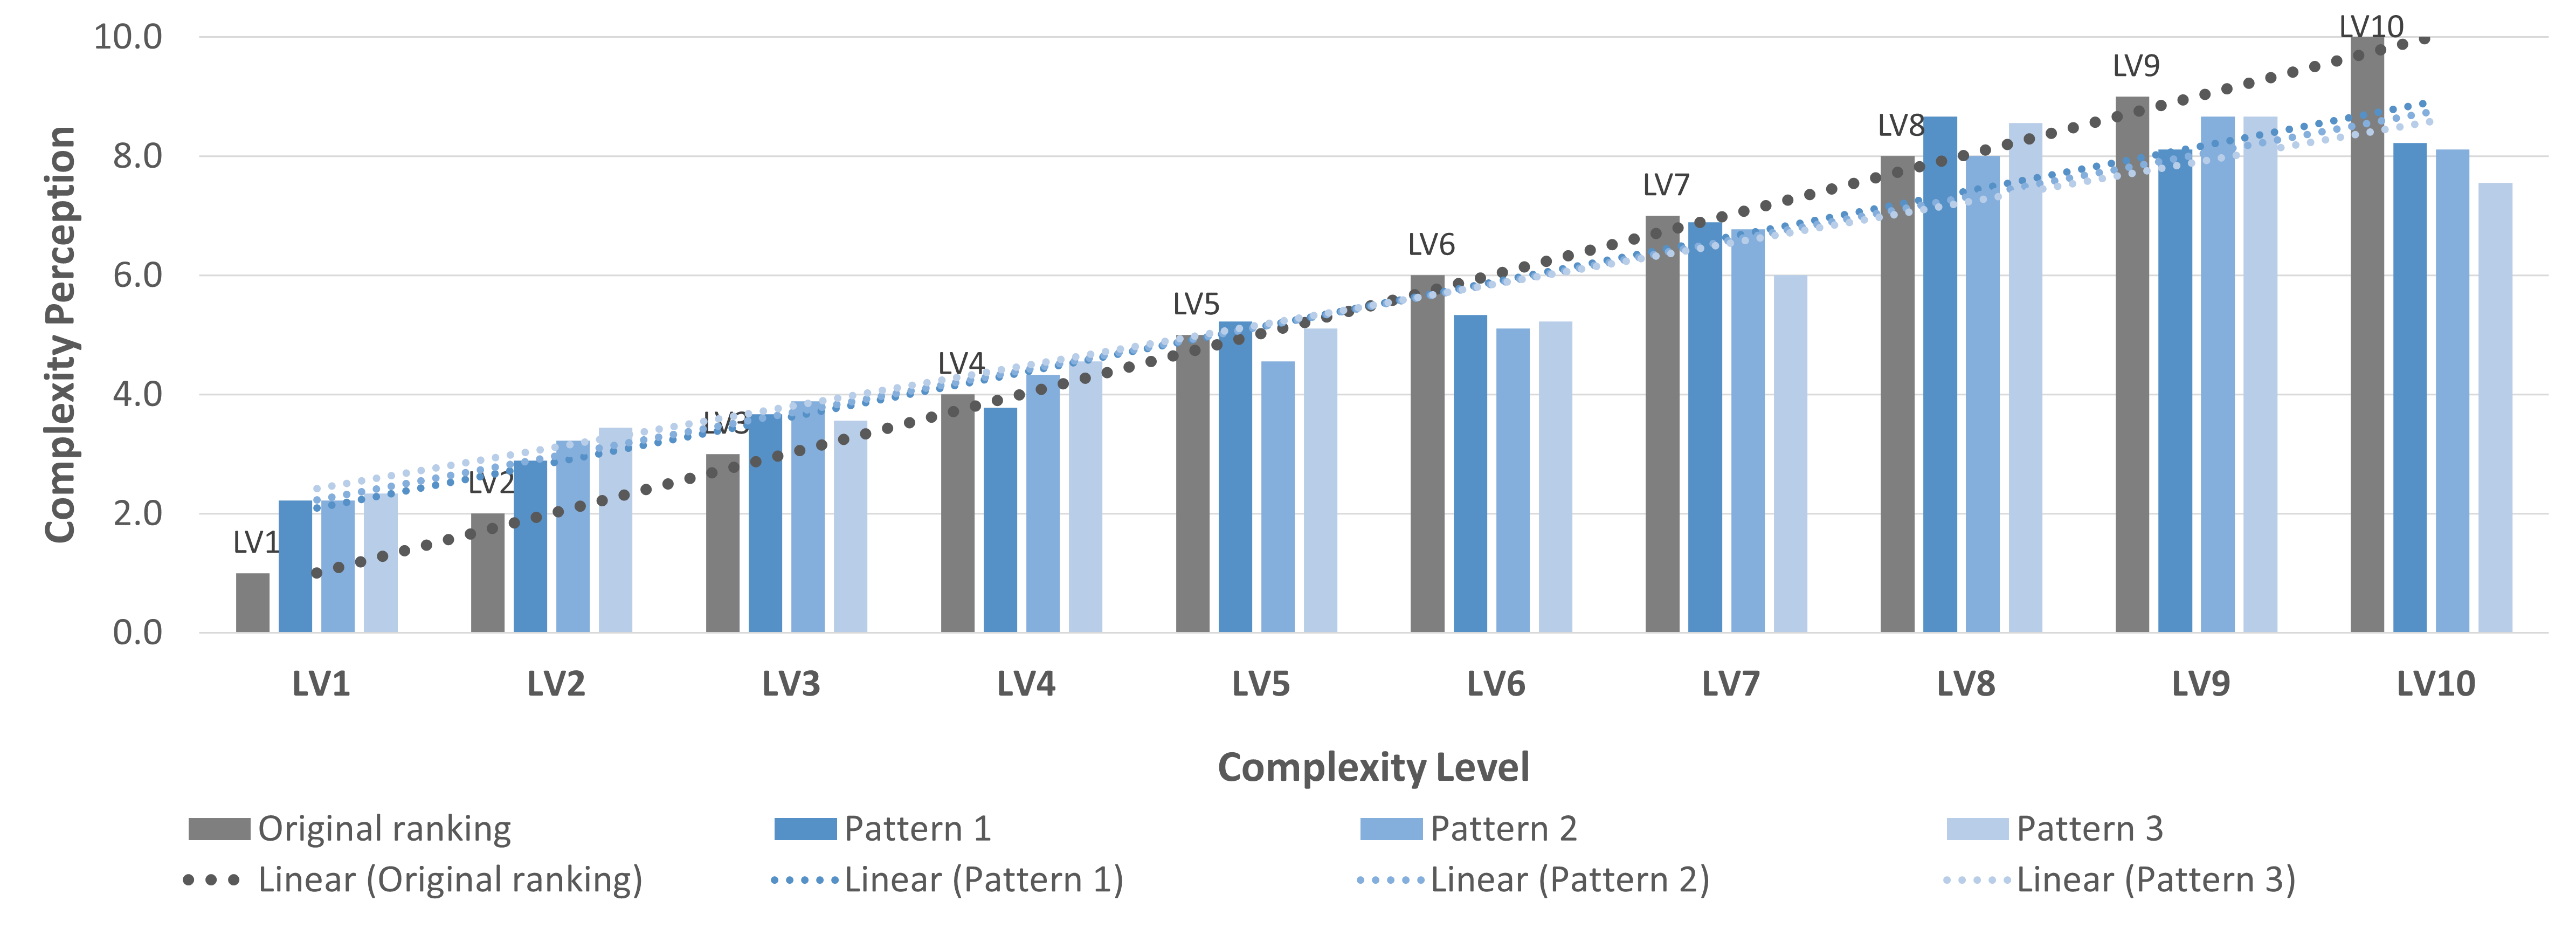
\includegraphics[width= \linewidth, trim=0 0 0 0]{Images/ComplexityPerceptionPerLevel}
      \caption{This graph highlights participants' perception of complexity for the 10 variations within three patterns in contrast to the original ranking. It visually represents the differences between participants' perceived complexity and the initial rankings during the screen-based complexity assessment stage of the experiment.}
      \label{fig:ComplexityPerceptionPerLevel2}
    \end{figure*}

% Old Figure Complexity perception Chart for all patterns
    \begin{figure}[htb]
        \centering
        %trim=100 180 100 120, clip
        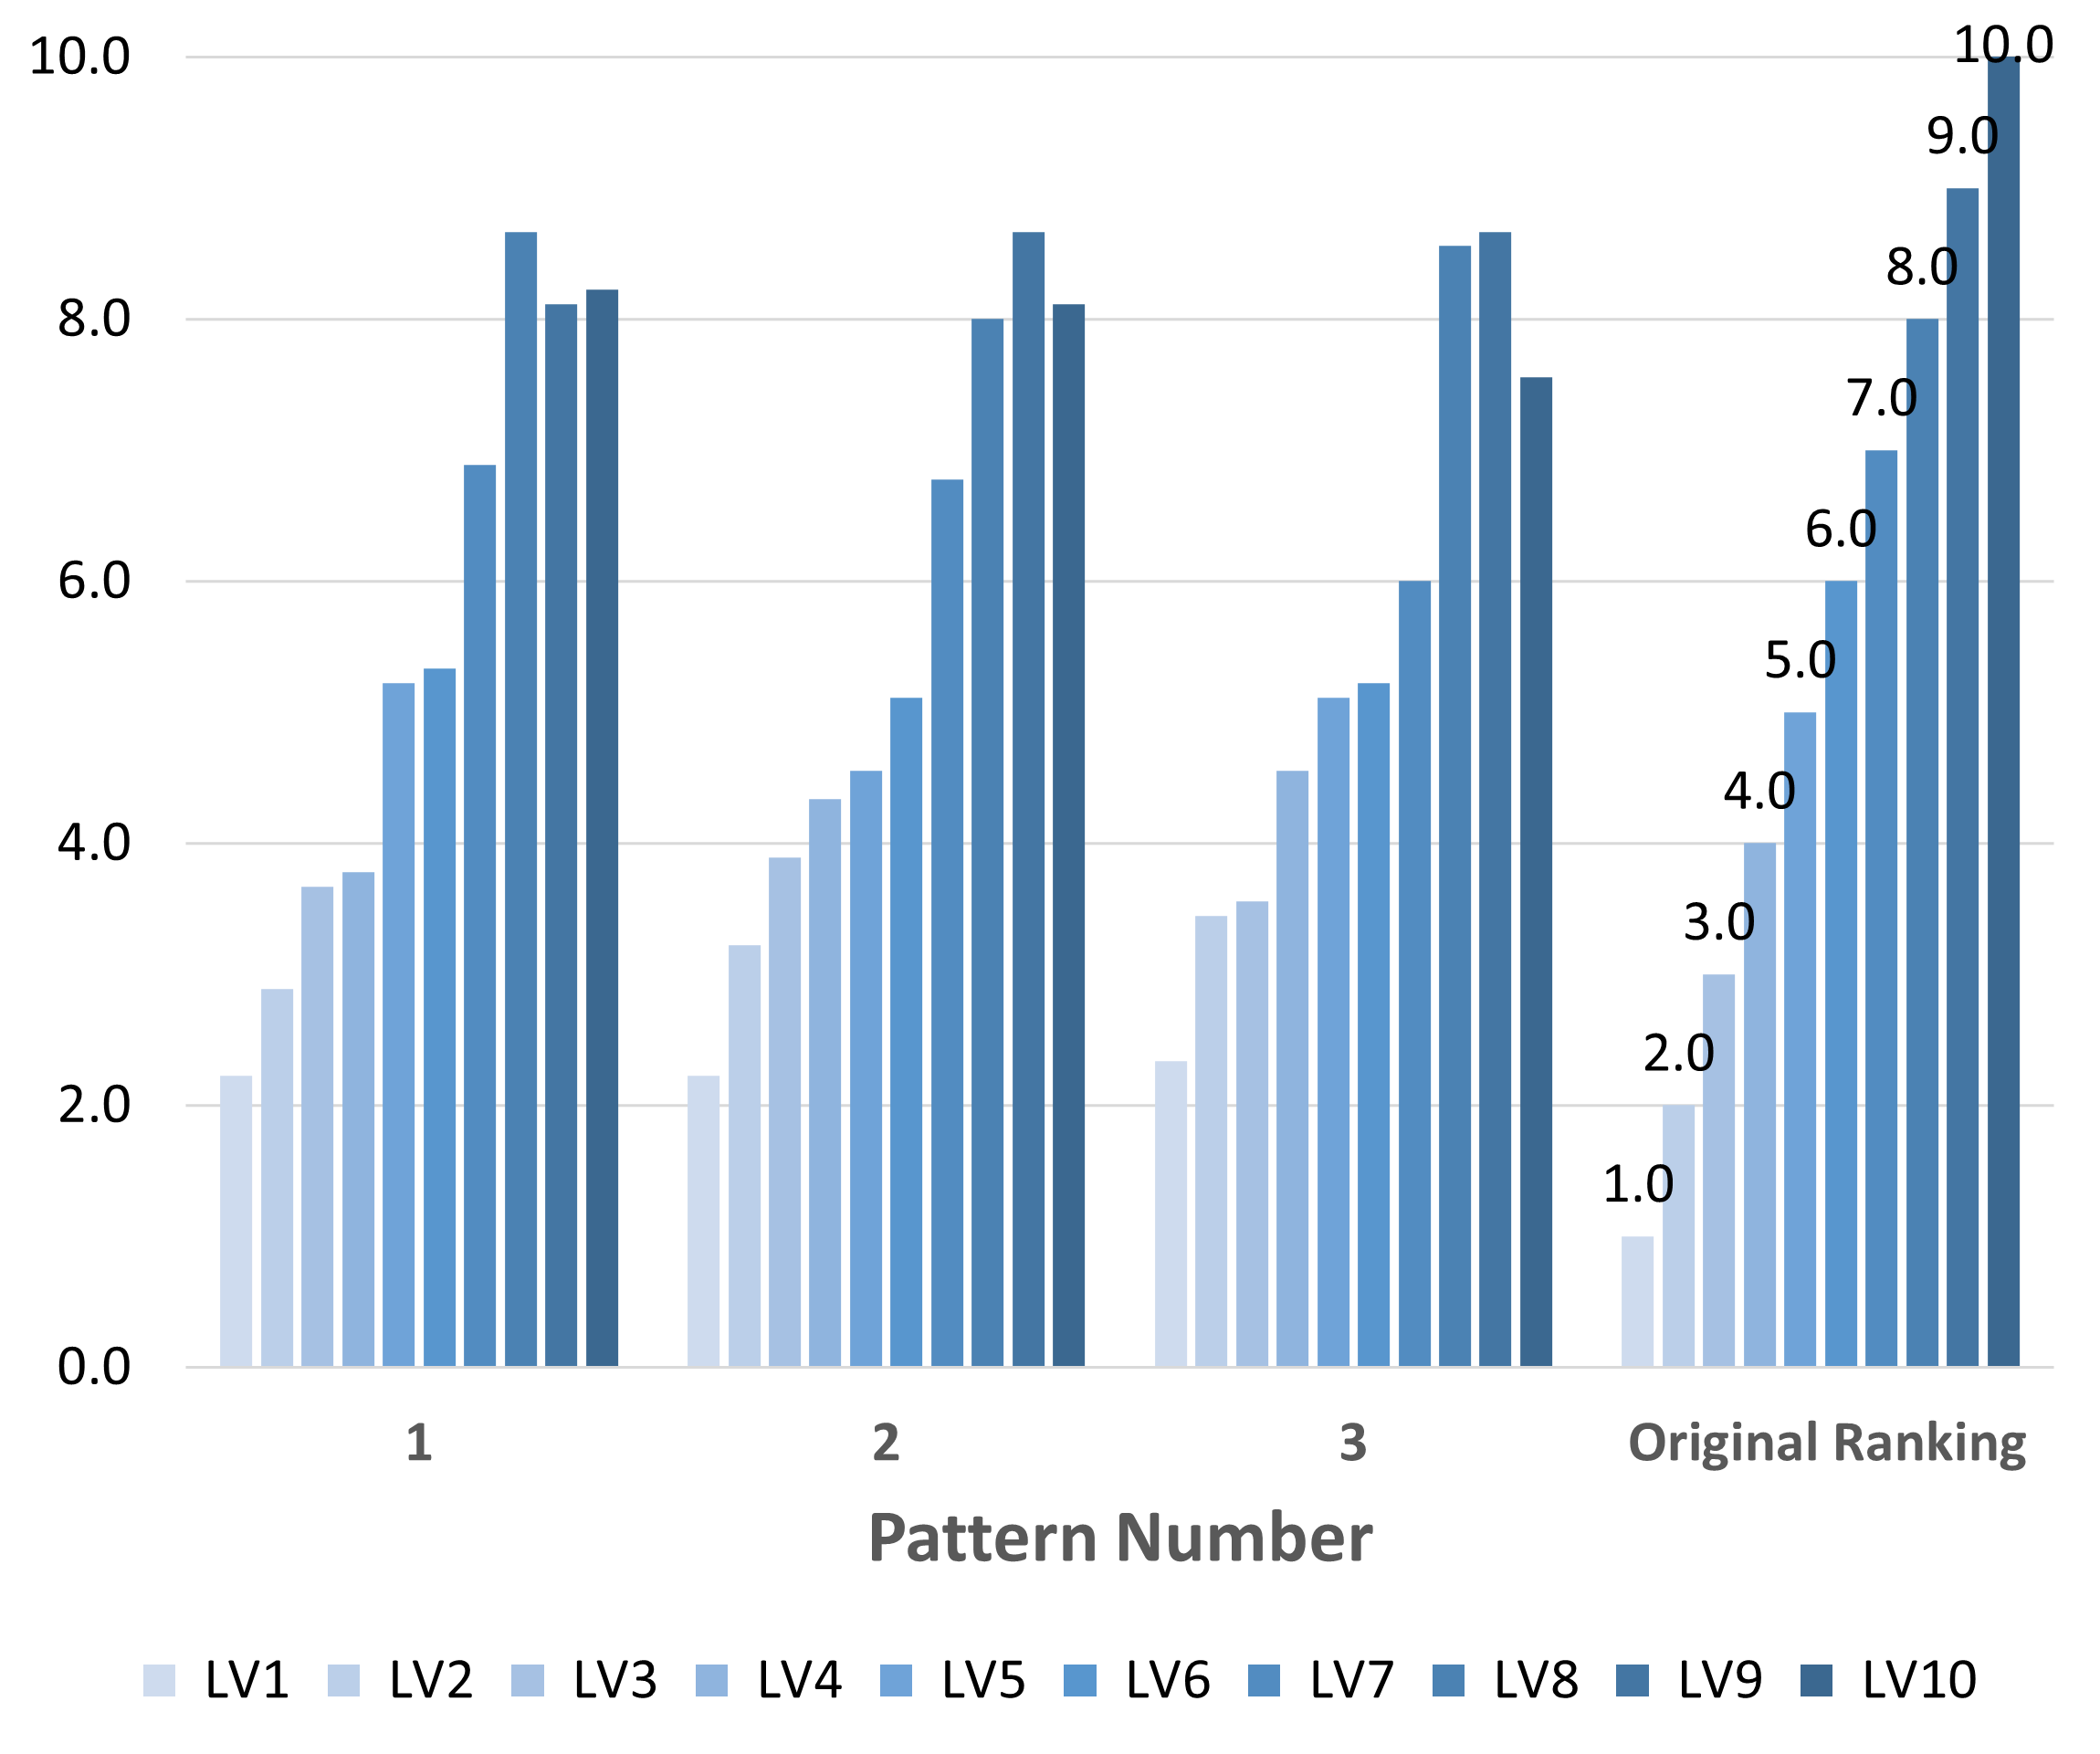
\includegraphics[width=\linewidth]{Images/ComplexityPerceptionChart}
        \caption{Chart depicting participants' complexity perception related to the three patterns. Insights into participants' perception of complexity concerning specific patterns during the screen-based complexity assessment phase of the experiment.}
        \label{fig:ComplexityPerceptionChart}
    \end{figure}


%! Future ornament graph

(Figure \ref{fig:complexornament})

%% Figure of Contemporary timeline
     \begin{figure*}[htb]
          \centering
          \includegraphics[width= \linewidth]{Images/complexornament}
          \caption{Complex ornament reference  (\textit{Images edited from source)}}
          \label{fig:complexornament}
        \end{figure*}




%! Texts

    %In Complexity and Contradiction in Architecture, Robert Venturi tries to give counter-arguments to the modernist approach. He advocates embracing ‘contradiction and Images’ to create valid, vital works.\cite{Lutolli2020}


    %It is noteworthy that he doesn’t oppose aesthetic simplicity. What he rejects is the ‘oversimplification’ of architecture, indicated when he inverted the famous Mies van der Rohe statement ‘Less is more’ into ‘Less is a bore’.\cite{Lutolli2020}

    %Modern architects, who shunned symbolism of form  as  an expression or reinforcement of content: meaning was  to  be  communicated,  not  through  allusion  to  previously  known forms, but through the inherent, physiognomic characteristics of form.
    %The creation of architectural form was to be a logical process, free  from images  of past experiences, determined solely by program and structure, with an  occasional  assist,  as  Alan Colquhoun has  suggested, from  intuition.
    But some recent critics  have  questioned  the possible level of content to  be derived  from  abstract forms.
    Others have  demonstrated that the functionalists,  despite  their protestations, derived  a  formal vocabulary of their own, mainly from current art movements and the industrial vernacular;
    and  latter-day  followers  such  as  the  Archigram  group  have turned,  while  similarly  protesting,  to Pop  Art and  the space  industry.\cite{Venturi1972}

   % Because the spatial relationships are made by symbols more than by forms, architecture in this landscape becomes symbol in space rather than form in space.
    Architecture defines very little: The big sign and the little building is the rule of Route 66.
    %The sign is more important than the architecture.
    %This is reflected in the proprietor's budget the sign at the front is a vulgar extravaganza, the building at the back, a modest necessity.
    The architecture is what is cheap.\cite{Venturi1972}

    %The commercial persuasion of road­side eclecticism provokes bold impact in the vast and complex setting of a  new landscape of big spaces, high speeds, and complex programs.\cite{Venturi1972}

    %parking lot is a current phase in the evolution of vast space since Versailles (Fig. 12). The space that divides high-speed highway and low, sparse buildings produces no enclosure and Iittle direction. \cite{Venturi1972}

    The little low buildings, gray-brown like the desert, separate and recede from the street that is now the highway, their false fronts disengaged and turned perpendicular to the highway as big, high signs.
    If you take the signs away, there is no place.
    The desert town is intensified communication along the highway.\cite{Venturi1972}

    Ugly and ordinary as symbol and style
    Heroic and Original, or ugly and ordinary

    %Robert Venturi, an iconoclastic architect often considered the father of postmodernism who rejected sterile, glass-cube structures in favor of an inclusive, eclectic style that embraced community values and a touch of vulgarity\cite{Schudel2018}

    He turned Mies van der Rohe’s famous dictum about simplicity in design — “Less is more” — upside down, cheekily declaring, “Less is a bore.”\cite{Schudel2018}

    Mr. Venturi’s declaration of architectural values, “Complexity and Contradiction,” was a manifesto that took aim at the prevailing modernist notion that architecture should aspire to a cold, glassy perfection with cold, glassy buildings.
    He argued instead that architecture should reflect changing times and social needs.
    The world of design, he said, had too long been in the grip of the dogma that architects were godlike creators who could impose their vision on the landscape.\cite{Schudel2018}

     Las Vegas wasn’t just a neon-lit den of vulgarity, they concluded.
     It was a prime example of a city built to accommodate the automobile.
     As a result, signs were often more important than the buildings they loomed over.\cite{Schudel2018}

    “In the landscape of the automobile, the architecture becomes insignificant, a pimple on the landscape of parking lots,” Mr. Venturi told the Times in 1971.\cite{Schudel2018}

    He never lost his disdain for what he considered the soulless architecture of his modernist predecessors, who often designed glass-box buildings with walls of windows, “but you would never have a wall with a window in it.”\cite{Schudel2018}

    Instead, Mr. Venturi wrote in “Complexity and Contradiction in Architecture,” he drew inspiration from the “everyday landscape, vulgar and disdained,” which was “valid and vital for our architecture as a whole.”\cite{Schudel2018}

    some architects wanted to move away from minimalist glass and steel and return to the ornamentation of the past. Postmodernists such as Michael Graves, James Stirling, Robert Venturi, and Denise Scott Brown responded to the work of their predecessors with bold buildings that showcased color and references to classical design. [...] Discover five of the most influential buildings of the postmodern movement and see how their eclectic and innovative designs pushed the boundaries of architecture in the 20th century\cite{Stamp2016}.

    Venturi wants modern architects to realize only one thing— perfection in the architectural world can and should include imperfection, in all its forms\cite{Lutolli2020}.

    %Modern architecture submerged symbolism. Instead it promoted expressionism, concentrating on the expression of architectural elements themselves: on the expression of structure and function\cite{Venturi1971}

    %Modern architecture's expression has become a dry expressionism, empty and boring. And in the end, irresponsible: i ron i c a I I y the Modern architecture of Crawford Manor, while rejecting explicit symbolism and frivolous applique ornament, has distorted the whole building into one big ornament\cite{Venturi1971}.

     Modern architects, who shunned symbolism of form  as  an expression or reinforcement of content: meaning was  to  be  communicated,  not  through  allusion  to  previously  known forms, but through the inherent, physiognomic characteristics of form.
    The creation of architectural form was to be a logical process, free  from images  of past experiences, determined solely by program and structure, with an  occasional  assist,  as  Alan Colquhoun has  suggested, from  intuition.
    But some recent critics  have  questioned  the possible level of content to  be derived  from  abstract forms.
    Others have  demonstrated that the functionalists,  despite  their protestations, derived  a  formal vocabulary of their own, mainly from current art movements and the industrial vernacular;
    and  latter-day  followers  such  as  the  Archigram  group  have turned,  while  similarly  protesting,  to Pop  Art and  the space  industry.\cite{Venturi1972}

    %
    According to Krier the mature city achieves balance with nature and with the people that it serves in its scale, size and integration of residential, commercial and civic functions.
    Krier argues that the reconstruction of a city is a moral imperative, a global project that it is at once cultural social economic and ecological. Time of video 1:06:29\cite{Economakis2023}